\documentclass[10pt,a4paper]{article}
\usepackage[utf8]{inputenc}
\usepackage{amsmath}
\usepackage{amsfonts}
\usepackage{amssymb}
\usepackage{amsthm}
\usepackage{float}
\usepackage{mathtools}
\usepackage{geometry}[margin=1in]
\usepackage{xspace}
\usepackage{tikz}
\usepackage{mathrsfs}
\usetikzlibrary{shapes, arrows, decorations.pathmorphing}
\usepackage[parfill]{parskip}
\usepackage{subcaption}
\usepackage{stmaryrd}
\usepackage{marvosym}
\usepackage{dsfont}

\newcommand{\st}{\text{ s.t. }}
\newcommand{\contr}{\lightning}
\newcommand{\im}{\mathfrak{i}}
\newcommand{\R}{\mathbb{R}}
\newcommand{\Q}{\mathbb{Q}}
\newcommand{\C}{\mathbb{C}}
\newcommand{\F}{\mathbb{F}}
\newcommand{\K}{\mathbb{K}}
\newcommand{\N}{\mathbb{N}}
\newcommand{\Z}{\mathbb{Z}}
\renewcommand{\H}{\mathds{H}}
\newcommand{\nequiv}{\not\equiv}
\newcommand{\powset}{\mathcal{P}}
\renewcommand{\th}[1][th]{\textsuperscript{#1}\xspace}
\newcommand{\from}{\leftarrow}
\newcommand{\legendre}[2]{\left(\frac{#1}{#2}\right)}
\newcommand{\ow}{\text{otherwise}}
\newcommand{\imp}[2]{\underline{\textit{#1.}$\implies$\textit{#2.}}}
\let\oldexists\exists
\renewcommand{\exists}{\oldexists\;}
\renewcommand{\hat}{\widehat}
\renewcommand{\tilde}{\widetilde}
\newcommand{\one}{\mathds{1}}
\newcommand{\under}{\backslash}
\newcommand{\injection}{\hookrightarrow}
\newcommand{\surjection}{\twoheadrightarrow}
\newcommand{\jacobi}{\legendre}
\newcommand{\floor}[1]{\lfloor #1 \rfloor}
\newcommand{\ceil}[1]{\lceil #1 \rceil}
\newcommand{\cbrt}[1]{\sqrt[3]{#1}}

\DeclareMathOperator{\ex}{ex}
\DeclareMathOperator{\id}{id}
\DeclareMathOperator{\upper}{Upper}
\DeclareMathOperator{\dom}{dom}

\DeclareMathOperator{\charr}{char}
\DeclareMathOperator{\Image}{im}
\DeclareMathOperator{\ord}{ord}
\DeclareMathOperator{\lcm}{lcm}
\let\emph\relax
\DeclareTextFontCommand{\emph}{\bfseries\em}

\newtheorem{theorem}{Theorem}[section]
\newtheorem{lemma}[theorem]{Lemma}
\newtheorem{corollary}[theorem]{Corollary}
\newtheorem{proposition}[theorem]{Proposition}
\newtheorem{conjecture}[theorem]{Conjecture}

\tikzset{sketch/.style={decorate,
 decoration={random steps, amplitude=1pt, segment length=5pt}, 
 line join=round, draw=black!80, very thick, fill=#1
}}

\title{Number Fields}
\begin{document}
\maketitle

\section{Algebraic Numbers and Algebraic Integers; Number Fields}
Here, we will use $F$ to denote any field containing $\Q$, for instance $F = \C$. Recall that an element $\alpha \in F$ is \emph{algebraic} (over $\Q$) if it is the root of some polynomial in $\Q[x]$. If so, there is a unique monic polynomial $m_{\alpha} \in \Q[x]$ of minimal degree with $m_{\alpha}(\alpha) = 0$, called the \emph{minimal polynomial} of $\alpha$. The \emph{degree} of $\alpha$ is the degree of $m_{\alpha}$

\begin{proposition}
Suppose $\alpha \in F$ is algebraic. Then $m_{\alpha}$ is irreducible in $\Q[x]$, and if $f \in \Q[x]$, then $f(\alpha) = 0 \iff m_{\alpha} | f$.
\end{proposition}
\begin{proof}
If $m_{\alpha} = fg$, then $f(\alpha)g(\alpha) = 0$, and since fields are integral domains we have $f(\alpha) = 0$ or $g(\alpha) = 0$. By minimality of degree, $f$ or $g$ is constant.

If $f(\alpha) = 0$, we write $f = gm_{\alpha} + h$, with $g, h \in \Q[x]$, and $\deg h < \deg m_{\alpha}$. Then $h(\alpha) = f(\alpha) - g(\alpha)m_{\alpha}(\alpha) = 0$, and so by minimality $h = 0$ and $m_{\alpha}|f$.

I.e. $\{f : f(\alpha) = 0\}$ is a principal ideal in $\Q[x]$ generated by $m_{\alpha}$
\end{proof}

If $\alpha \in F$, define $\Q(\alpha)$ to be the smallest subfield of $F$ containing $\alpha$. Explicitly, it can be shown that $\Q(\alpha) = \left\{ \frac{f(\alpha)}{g(\alpha)} : f, g \in \Q[x], g(\alpha) \neq 0\right\}$.

\begin{proposition}
If $\alpha \in F$ is algebraic of degree $n$, then $1, \alpha, \ldots, \alpha^{n-1}$ is a $\Q$-basis for $\Q(\alpha)$. Conversely, if $[\Q(\alpha): \Q] \coloneqq \dim_{\Q} \Q(\alpha)$ is finite, say $n$, then $\alpha$ is algebraic of degree $n$.
\end{proposition}
\begin{proof}
Consider the homomorphism $\phi:\Q[x] \to F; f\mapsto f(\alpha)$. Then $\ker(\phi) = (m_\alpha)$ which is maximal, so $\Image \phi$ is a field, and hence equal to $\Q(\alpha)$. As $\deg m_{\alpha} = n$, a basis for $\Q[x]/(m_\alpha)$ is $1, x, \ldots, x^{n-1}$, and hence $1, \alpha, \ldots, \alpha^{n-1}$ is a basis for $\Q(\alpha)$.

For the converse part, if $[\Q(\alpha):\Q] = n < \infty$, then $1, \alpha, \ldots, \alpha^n$ are linearly dependent and so $\alpha$ is algebraic of some degree. By the first part, this degree is $n$.
\end{proof}

\begin{proposition}
$\{\alpha \in F : \alpha$ algebraic$\}$ is a subfield of $F$.
\end{proposition}
\begin{proof}[Galois theory]
It is enough to prove that it is closed under $+, \times$ and inverse. For $+$ and $\times$ see \textbf{1.6} below for a stronger statement. If $0 \neq \alpha$ is algebraic, then $\sum^n b_j \alpha^j = 0 \implies \sum^n b_{n-j}(\alpha^{-1})^j = 0$, and so $\alpha^{-1}$ is algebraic.
\end{proof}

$\alpha \in F$ is an \emph{algebraic integer} if there is a monic polynomial $f \in \Z[x]$ with $f(\alpha) = 0$.
\stepcounter{theorem}

\begin{lemma}
\item
\begin{enumerate}
\item Let $\alpha \in F$. Then the following are equivalent:
\begin{enumerate}
\item $\alpha$ is an algebraic integer
\item $\alpha$ is algebraic and $m_\alpha \in \Z[x]$
\item $\Z[\alpha]$ is a finitely generated $\Z$-module
\end{enumerate}
If these hold, then $1, \alpha, \ldots, \alpha^{d-1}$ is a $\Z$-bases for $\Z[\alpha]$, with $d = \deg \alpha$.
\item $\alpha \in \Q$ is an algebraic integer $\iff \alpha \in \Z$
\end{enumerate}
\end{lemma}
Recall the notation that, if $\alpha_1, \ldots, \alpha_n \in F$, then $\Z[\alpha_1, \ldots, \alpha_n]$ is the smallest subring of $F$ containing $\{\alpha_i:i\in[n]\}$, i.e. the set of all finite sums of terms of the form $A\alpha_1^{i_1}\ldots\alpha_n^{i_n}$ for $A, i_1, \ldots, i_n \in \Z$.

\begin{proof}\item
\begin{enumerate}
\item
\begin{enumerate}
\imp{a}{b} Suppose $f(\alpha) = 0, f \in \Z[x]$, $f$ monic. Then \textbf{1.1} gives that $f = gm_{\alpha}$ for some $g \in \Q[x]$ necessarily monic. Gauss's lemma from GRM gives us that $m_{\alpha}, g$ are in $\Z[x]$.

\imp{b}{c} Write $m_{\alpha} = x^d + \sum_{j=1}^{d-1} b_j x^j$, for $b_j \in \Z$. Then $\alpha^d = -\sum_{j=1}^{d-1} b_j \alpha^j$, from which we say that every $\alpha^n$ is a $\Z$-linear combination of $1, \alpha, \ldots, \alpha^{d-1}$. So $\Z[\alpha]$ is generated by $1, \alpha, \ldots, \alpha^{d-1}$ as a $\Z$-module. There is no linear relation between $1, \alpha, \ldots, \alpha^{d-1}$, as $d = \deg \alpha$. So $\Z[\alpha]$ is finitely generated and $1, \alpha, \ldots, \alpha^{d-1}$ is a $\Z$-basis.

\imp{c}{a} Assume $\Z[\alpha]$ is finitely generated by $g_1(\alpha), \ldots, g_r(\alpha)$. For some $g_i \in \Z[x]$. Let $k = \max\{\deg g_i\}$. Then $\Z[\alpha]$ is certainly generated by $1, \alpha, \ldots, \alpha^k$ as a $\Z$-module. So $\alpha^{k+1} = \sum_{j=0}^k b_j \alpha^j$ for $b_j \in \Z$, and so $\alpha$ is an algebraic integer.
\end{enumerate}
\item $\alpha \in \Q \implies m_{\alpha} = x-\alpha$, and so $\alpha$ is an algebraic integer $\iff \alpha \in \Z$ using $(a) \iff (b)$.
\end{enumerate}
\end{proof}

\begin{theorem}
If $\alpha, \beta \in F$ are algebraic integers, then so are $\alpha\beta, \alpha\pm\beta$.
\end{theorem}
\begin{proof}
The $\Z$-module $\Z[\alpha,\beta]$ is generated by $\{\alpha^i\beta^j : 0 \leq i < \deg \alpha; 0 \leq j < \deg \beta\}$, and so is finitely generated. Hence so is the submodule $\Z[\alpha\beta]\subseteq \Z[\alpha,\beta]$. So $\alpha\beta$ is an algebraic integer by \textbf{1.4}. The same applies for $\alpha+\beta, \alpha-\beta$.
\end{proof}

Now to introduce the main characters of this course:

An \emph{algebraic number field} (or just \emph{number field}) is a field $K \supset \Q$ which is a finite extension, i.e. $[K:\Q] < \infty$. The \emph{ring of integers of K}, written $\o_K$, is the set of algebraic integers in $K$. By \textbf{1.6} it is a ring. It is useful to have the converse:

\begin{proposition}
Let $\alpha \in F$ be algebraic. Then for some $0 \neq b \in \Z, b\alpha$ is an algebraic integer.
\end{proposition}
\begin{proof}
Exercise.
\end{proof}

\begin{theorem}[Primitive Element]
If $K$ is a number field, then $K = \Q(\alpha)$ for some $\alpha \in K$.
\end{theorem}
\begin{proof}
Done in Galois theory.
\end{proof}

\section{Quadratic Fields}
$K$ is a \emph{quadratic field} if $[K:\Q] = 2$. In this case, let $\alpha \in K \setminus \Q$. The minimal polynomial $m_{\alpha}$ is a quadratic, and so solving we get $\alpha = x+\sqrt{y}\footnote{By $\sqrt{y}$ we just mean some $\beta \in K$ with $\beta^2 = y$}$ for $x,y \in \Q, y \neq 0$. Since $y$ is not a rational square, we can write $y$ uniquely as $z^2 d$ for $z \in \Q\setminus\{0\}$, $d\neq 0,1$ a square-free integer. So $K = \Q(\sqrt{d}) = \Q[x]/(x^2-d)$. If $d' \neq d$ also square-free, then $\Q(\sqrt{d}) \ncong \Q(\sqrt{d'})$.

Now we want to compute $\o_K$. Let $\alpha = u + v\sqrt{d} \in K$ for $u, v \in \Q$. If $v = 0, \alpha \in \o_K \iff \alpha \in \Z$. Otherwise, $\alpha \notin \Q$, and $m_{\alpha} = x^2 - 2ux + (u^2-dv^2)$. So $\alpha \in \o_{K} \iff 2u \in \Z$ and $u^2-dv^2 \in \Z$.

If $u \in \Z$, then $dv^2 \in \Z$, and since $d$ is square-free, we must have $v \in \Z$. Otherwise, $u = \frac{2a+1}{2}, a \in \Z$, and we must have $4dv^2 - (2a+1)^2 \in 4\Z$, which holds if and only if $v = \frac{k}{2}, k \in \Z$ and $dk^2 \equiv 1 \mod 4$. If $d \equiv 1 \mod 4$, this holds if and only if $k$ is odd, and if $d$ is not $1\mod 4$, then this congruence cannot hold.

In conclusion,
\begin{theorem}
If $d \in \Z\setminus\{0,1\}$ is square-free, and $K = \Q(\sqrt{d})$, then:
\begin{enumerate}
\item If $d \nequiv 1 \mod 4$, then $\o_K = \{u + v\sqrt{d} : u, v \in \Z\} = \Z[\sqrt{d}]$.
\item If $d \equiv 1 \mod 4$, then $\o_K = \{u + v\sqrt{d}: u, v \in \frac12\Z, u-v\in \Z\} = \Z[\frac{1+\sqrt{d}}{2}]$
\end{enumerate}
\end{theorem}

\underline{Examples:} If $d = -3$, then $\o_{\Q(\sqrt{-3})} = \Z[\frac{1+\sqrt{-3}}{2}] = \Z[\xi_3]$.

Note that, for a general number field $K$, we needn't have $\o_K = \Z[\alpha]$ for $\alpha \in K$, and in fact for $\deg K > 2$ this method is unlikely to be practical for computing $\o_K$.

\section{Embeddings}
Let $K$ be a number field with $[K:\Q] = n$.

\begin{theorem}
There are precisely $n$ homomorphisms $\sigma_i:K \injection \C$. These are called the \emph{complex embeddings} of $K$. More generally, if $\Q\subset F\subset K$ are number fields, then each of the $[F:\Q]$ complex embeddings of $F$ extend to exactly $[K:F]$ complex embeddings of $K$.
\end{theorem}
\begin{proof}[Proof. (Galois Theory)]
Assume $K = \Q(\theta) = \Q[x]/(m_\theta)$ by the theorem of the primitive element. Then to give $\sigma: K \injection \C$ is the same as to give $\phi:\Q[x]\to \C$ with $\phi(m_{\theta}) = 0$. If $z = \phi(x)$, then $\phi(m_\theta) = m_\theta(z)$, giving a bijection $\{\sigma:K \injection \C\} \leftrightarrow \{$roots of $m_{\theta} \in \C\}$, coming from $\sigma \mapsto \sigma(\theta)$. The second part is the same as the first, but replacing $\Q$ by $F$ since $\theta$ has degree $[K:F]$ over $F$.
\end{proof}

\underline{Remarks:}
\begin{enumerate}
\item If $K \subset \C$ we can choose $\sigma$ to be the inclusion.
\item For some $r \in \{0, \ldots, n\}$, exactly $r$ of the $\sigma_{i}$ will be \emph{real}, i.e. $\sigma_{i}(K) \subseteq \R$. The remaining embeddings will then come in complex conjugate pairs $\sigma_i, \overline{\sigma_i}$. So $n = r+2s$, where $r$ is the number of real embeddings, and $s$ is the number of complex conjugate pairs of embeddings.
\end{enumerate}\newpage

\hspace*{-1em}\underline{Examples:} 
\begin{itemize}
\item[$\Q(\sqrt{d})$.] We have two cases:
\begin{itemize}
\item[$d>0$.] There are $2$ real embeddings: $\sigma_1:\sqrt{d} \mapsto +\sqrt{d} \in \R$, and $\sigma_2:\sqrt{d} \mapsto -\sqrt{d} \in \R$. So $(r,s) = (2, 0)$.
\item[$d<0$.] There is now one pair of complex embeddings, given by $\sigma_1:\sqrt{d} \to \im \sqrt{|d|}; \sigma_2:\sqrt{d}\to -\im\sqrt{|d|}$. So $(r,s) = (0,1)$.
\end{itemize}
\item[$\Q(\cbrt{2})$.] We have 1 real embedding $\cbrt{2} \mapsto \cbrt{2} \in \R$, and the two complex embeddings $\cbrt{2} \mapsto \omega^{\pm 1}\cbrt{2} \in \C$, so $(r, s) = (1,1)$.
\end{itemize}

\begin{proposition}
If $\alpha \in K$, then the complex numbers $\sigma_i(\alpha)$ are the complex roots of $m_\alpha$, each taken $n/\deg(\alpha)$ times.
\end{proposition}
\begin{proof}
Apply the 2\th[nd] part of \textbf{3.1} with $F = \Q(\alpha)$.
\end{proof}

\section{Norm and Trace}
Given $K$ a number field, $\alpha \in K$, define a map $u_{\alpha}: K \to K$ by $u_{\alpha}(x) = \alpha x$. $K$ is a $\Q$-vector space, and $u_{\alpha}$ is a $\Q$-linear map.  Define:
\begin{itemize}
\item $f_{\alpha}$ to be the \emph{characteristic polynomial} of $u_{\alpha}$, so $f_{\alpha} = \det(x-u_{\alpha}) \in \Q[x]$, monic
\item $\Nn_{K/\Q}(\alpha) = \det(u_{\alpha}) \in \Q$, the \emph{norm} of $\alpha$
\item $\Tr_{K/\Q}(\alpha) = \tr(u_{\alpha}) \in \Q$, the \emph{trace} of $\alpha$ 
\end{itemize}
More explicitly, let $\beta_1, \ldots, \beta_n$ be a $\Q$-basis for $K$. Then $\alpha\beta_i = \sum_{j=1}^n A_{ji}\beta_j$ for some $A \in M_{n,n}(\Q)$. Then $f_{\alpha} = \det(x\cdot I_n - A), \Nn_{K/\Q}(\alpha) = \det(A), \Tr_{K/\Q} = \tr(A)$. As an exercise, work these out for $\Q(\sqrt{d})$.

\begin{proposition}
\begin{align*}
\Nn_{K/\Q}(\alpha\beta) &= \Nn_{K/\Q}(\alpha)\Nn_{K/\Q}(\beta)\\
\Tr_{K/\Q}(\alpha+\beta) &= \Tr_{K/\Q}(\alpha) + \Tr_{K/\Q}(\beta)
\end{align*}
\end{proposition}
\begin{proof}
From the definition, $u_{\alpha\beta} = u_{\alpha}u_{\beta}$, and $u_{\alpha+\beta} = u_{\alpha} + u_{\beta}$, so the result follows from linear algebra.
\end{proof}

\begin{theorem}
\item
\begin{enumerate}
\item The minimal polynomial of $u_{\alpha}$ is $m_{\alpha}$, and $f_{\alpha} \prod_{i=1}^n(x-\sigma_i(\alpha)) = m_{\alpha}^{n/d}$, where $\deg(\alpha) = d$.

\item $\Nn_{K/\Q}(\alpha) = \prod_{i=1}^n \sigma_i(\alpha), \Tr_{K/\Q}(\alpha) = \sum_{i=1}^n \sigma_i(\alpha)$.
\end{enumerate}
We call the $\sigma_i(\alpha)$ the \emph{conjugates} of $\alpha$.
\end{theorem}
\begin{proof}
Note that \textit{1.}$\implies$\textit{2.}, because $\det u_{\alpha} = (-1)^n f_{\alpha}(0)$, the product of the eigenvalues, and $\tr u_{\alpha} = -($coeff. of $ x^{n-1}$ in $f_\alpha)$.

For \textit{1.}, we first do the case $\deg \alpha = n$, i.e. $K = \Q(\alpha)$. Then $f_\alpha, m_\alpha \in \Q[x]$ are monic of degree $n$, and if $\beta \in K$ then $f_{\alpha}(\alpha)\beta = f_{\alpha}(u_{\alpha})\beta = 0$ by Cayley-Hamilton. So $f_\alpha(\alpha) = 0 \implies m_\alpha = f_\alpha$.

In general, if $[K:\Q(\alpha)] = \frac{n}{d}$, then $K \cong \Q(\alpha)^{\oplus(n/d)}$, and then $f_\alpha = ($char. poly. of $u_\alpha$ on $\Q(\alpha))^{n/d} = m_\alpha^{n/d} = \prod_{i=1}^n (x-\sigma_i(\alpha))$.
\end{proof}
\begin{corollary}
\item
\begin{enumerate}
\item Let $\alpha \in K$. Then $\alpha = 0 \iff \Nn_{K/\Q}(\alpha) = 0$.
\item Let $\alpha \in \o_K$. Then $f_{\alpha} \in \Z[x]$, and $\Nn_{K/\Q}(\alpha), \Tr_{K/\Q}(\alpha) \in \Z$. Moreover, $\Nn_{K/\Q}(\alpha) \in \{\pm 1\}$ if and only if $\alpha \in \o_k^{\ast}$ is a \emph{unit}, i.e. $\alpha^{-1} \in \o_k$.
\end{enumerate}
\end{corollary}
\begin{proof}
\item
\begin{enumerate}
\item $\alpha = 0 \iff \sigma_i(\alpha) = 0$ for all $i$.
\item $m_\alpha \in \Z[x]$, so $f_\alpha \in \Z[x]$, and hence $\Nn_{K/\Q}(\alpha), \Tr_{K/\Q}(\alpha) \in \Z$, since they are coefficients of $f_{\alpha}$ up to a choice of sign. 

If $\alpha$ is a unit, then $\Nn_{K/\Q}(\alpha)\Nn_{K/\Q}(\alpha^{-1}) = \Nn_{K/\Q}(\alpha\alpha^{-1}) = \Nn_{K/\Q}(1) = 1$, and so $\Nn_{K/\Q}(\alpha)$ is a unit and an integer, so in $\{\pm 1\}$.

If $\Nn_{K/\Q}(\alpha) \in \{\pm 1\}, f_\alpha = x^n + \sum_{i=1}^{n-1} b_i x^i \pm 1$, so $f_\alpha(\alpha) = 0 \implies \alpha\cdot\left(\alpha^{n-1}+\sum_{i=1}^{n-1}b_i\alpha^{i-1}\right) = \mp 1$, so $\alpha^{-1} \in \o_K$ and we have an explicit representation of $\alpha^{-1}$.
\end{enumerate}
\end{proof}

Note that we can also define, if $\Q \subset F \subset K$ the relative trace $\Tr_{K/F}(\alpha), \Nn_{K/F}(\alpha)$ as the trace/determinant of $u_{\alpha}$ viewed as an $F$-linear map from $K \simeq F^{[K:F]}$ to itself, and we have that:
\begin{align*}
\Tr_{K/\Q} = \Tr_{F/\Q}\cdot\Tr_{K/F}\;\;\;\;\;\;\;\;\; \Nn_{K/\Q} = \Nn_{F/\Q}\cdot\Nn_{K/F}
\end{align*}

\section{Some Modules from GRM}
\begin{proposition}
$G$ is a finitely generated abelian group written additively with no torsion, i.e. no elements of finite order, and a finite set of generators $x_1, \ldots, x_n$. Let $H \subset G$ be the subgroup generated by $y_1, \ldots, y_n \in G$, where $y_i = \sum_{j=1}^n A_{ji}x_j$ for some $A \in Mat_{n,n}(\Z)$ Then if $\det(A) \neq 0$, $H$ has finite index in $G$, with $(G:H) = |\det A|$.
\end{proposition}
\begin{proof}
Using Smith normal form, $A = PDQ$ for $P,Q,D$ integer $n\times n$ matrices where $\det P, \det Q \in \{\pm 1\}$ and $D = diag(d_1, \ldots, d_n)$ for $d_i \geq 0$, $d_i | d_{i+1}$. Then $G/H \cong \Z/d_1\Z \times \ldots \times \Z/d_n\Z$, where $\Z/0\Z = \Z$.

Hence if $|\det A| = \prod_i d_i \neq 0$, then $G/H$ contains no $\Z$ terms and has dimension $\prod_i d_i = |\det A|$.
\end{proof}

Let $V$ be a $\Q$-vector space, and $\dim(V) = n < \infty$. Let $H \subset V$ be a subgroup, viewed as a sub-$\Z$-module. Then define:
\begin{align*}
\rank(H) = \dim(\spann(H)) \in \{0, 1, \ldots, n\}
\end{align*}
\begin{proposition}
If $H$ is finitely generated as an abelian group then $H = \bigoplus_{i=1}^r \Z v_i$ where $r = \rank(H)$ and $x_1, \ldots, x_r \in V$ are linearly independent.
\end{proposition}
\begin{proof}
$H$ has no torsion as $V$ is a $\Q$-vector space, so by classification $H$ is an abelian group freely generated by some $x_1, \ldots, x_r$. If $a_i \in \Q$ and $\sum a_i x_i = 0$ in $V$, then clearing denominators we have $\sum b_i x_i = 0$ with $b_i \in \Z$. So we must have $b_i = 0$ for all $i$, so $a_i = 0$ and the $x_i$ are linearly independent, and $r = \rank(H)$ by the definition of rank.
\end{proof}

\section{Discriminants and Integral Bases}
Let $\alpha_1, \ldots, \alpha_n \in K$. Define the \emph{discriminant}
\begin{align*}
\Disc(\alpha_1) = \Disc(\alpha_1, \ldots, \alpha_n) = \det(\Tr_{K/\Q}(\alpha_i\alpha_j))) \in \Q
\end{align*}
\begin{theorem}
\item
\begin{enumerate}
\item $\Disc(\alpha_1, \ldots, \alpha_n) = \det(\sigma_i(\alpha_j))^2$.
\item $\Disc(\alpha_i) \neq 0  \iff \alpha_1, \ldots, \alpha_n$ is a $\Q$-basis for $K$.
\item If $\beta_i = \sum_{j=1}^n A_{ji}\alpha_j$ for $A \in Mat_{n,n}(\Q)$, then $\Disc(\beta_i) = (\det A)^2\Disc(\alpha_i)$
\item Suppose $(\alpha_i)$ is a $\Q$-basis. Then $\Disc(\alpha_i)$ depends only on the subgroup $\Z\alpha_1+\ldots+\Z\alpha_n \in K$.
\end{enumerate}
\end{theorem}
\begin{proof}
\item
\begin{enumerate}
\item Let $\Delta = (\sigma_i(\alpha_j))_{ij} \in Mat_{n,n}(\C)$. Then $(\Delta^\intercal\Delta)_{ij} = \sum_{k=1}^n \sigma_k(\alpha_i)\sigma_k(\alpha_j) = \sum_{k=1}^n \sigma_k(\alpha_i\alpha_j) = \Tr_{K/\Q}(\alpha_i\alpha_j)$

So $(\det \Delta)^2 = \det(\Delta^\intercal\Delta) = \det\Tr_{K/\Q}(\alpha_i\alpha_j)$.

\item If $\alpha_1, \ldots, \alpha_n$ is not a $\Q$-basis, then there are some $b_1, \ldots, b_n \in \Q$, not all $0$, with $\sum b_j\alpha_j = 0$. Then for all $i$, $0 = \sigma_i\left(\sum_{j=1}^n b_j\alpha_j\right) = \sum_{j=1}^n b_j\sigma_i(\alpha_j)$, so $\det \Delta = 0$, hence $\disc(\alpha_i) = 0$.

For the other direction, suppose $(\alpha_i)$ is a $\Q$-basis for $K$, and let $T = (\Tr_{K/\Q}(\alpha_i\alpha_j))_{ij}$. It is enough to prove that, for $b \in \Q^n\setminus\{0\}, Tb \neq 0$, or equivalently that there is $c \in \Q^n$ such that $c^\intercal Tb \neq 0$. But if $\beta  = \sum_j jb_j\alpha_j, \gamma = \sum_j c_j\alpha_j$, then $c^\intercal T b = \sum_{i,j} c_i \Tr_{K/\Q}(\alpha_i\alpha_j)b_j = \Tr_{K/\Q}(\sum_{i,j}c_ib_j\alpha_i\alpha_j ) = \Tr_{K/\Q}(\beta\gamma)$, so taking $\gamma = \frac1\beta$, we get $\Tr_{K/\Q}(1) = n \neq 0$.

\item $\Delta = (\sigma_i(\alpha_j)), \Delta' = (\sigma_i(\beta_j))$, so $\Delta'_{ij} = \sum_k \sigma_i(A_{kj}\alpha_k) = \sum_{k} A_{kj}\sigma_i(\alpha_k) = (\delta A)_{ij}$. Hence $\det \Delta' = \det \Delta \det A$, and result follows by part 1.

\item If $(\alpha_i), (\beta_i)$, generate the same subgroup, then $\beta_i = \sum A_{ji}\alpha_j$, where $A_{ij} \in \Z, \det A \in \{\pm 1\}$. Then by part 3, $\Disc(\beta_i) = (\det A)^2 \Disc(\alpha_i) = \Disc(\alpha_i)$.
\end{enumerate}
\end{proof}


If $H \subset K$ is a finitely generated subgroup of rank $n$, and $(\alpha_1, \ldots, \alpha_n)$ is a $\Z$-basis for $H$, then above implies that $\Disc(\alpha_1, \ldots, \alpha_n)$ is a non-zero rational, depending only on $H$, which we call $\Disc(H)$.

\begin{lemma} If $H \subset H' \subset K$ are finitely generated subgroups of rank $n$, then
\begin{align*}
\Disc(H) = (H':H)^2\Disc(H')
\end{align*}
\end{lemma}
\begin{proof}
Pick $\Z$-bases $(\alpha_i), (\alpha_i')$ for $H, H'$. Then $\alpha_i = \sum_j B_{ji} \alpha'_j$, for $B \in Mat_{n,n}(\Z)$. Then by \textbf{6.1}\textit{(3.)}, together with \textbf{5.1}, give that:
\begin{align*}
(H':H)^2 = (\det B)^2 = \Disc(H)/\Disc(H')
\end{align*}
\end{proof}

\begin{theorem}
There exist $\omega_1, \ldots, \omega_n \in \o_K$ such that $\o_K = \Z\omega_1\oplus\ldots\oplus\Z\omega_n$ (i.e. that $\o_K$ is finitely generated as a $\Z$-module). We say that $(\omega_i)$ is an \emph{integral basis} for $K$.
\end{theorem}
\begin{proof}
Certainly, there is $\omega_1, \ldots, \omega_n \in \o_K$ which form a $\Q$-basis for $K$ - take any $\Q$-basis of $K$ and multiply by a suitable non-zero integer. Then for such a basis, $\Disc(H) \in \Z\setminus\{0\}$ where $H = \sum_i \Z\omega_i \subset K$.

Choose such a basis with $|\Disc(H)|$ minimal. Then let $\alpha \in \o_K$, and let $H' = \Z\alpha + H \subset K$. Then $H' \subset H$ are finitely generated of rank $n$, and so by \textbf{6.2}, $\Disc(H) = (H':H)^2\Disc(H')$, and by minimality of $\Disc(H), H' = H$, so $\alpha \in H$.
\end{proof}

The \emph{discriminant of K} $d_K = \Disc(\o_K) = \Disc(\omega_i)$ for any integral basis $(\omega_i)$.

\hspace*{-1em}\underline{Example:} Let $K = \Q(\sqrt{d})$ for $d$ a square free integer not 0 or 1.
\begin{itemize}
\item[$d \nequiv 1 \mod 4$:] An integral basis is $\{1, \sqrt{d}\}$ and so we have $\Delta = (\sigma_i(\alpha_k)) = \begin{pmatrix} 1 & \delta \\ 1 & -\delta\end{pmatrix}$, where $\sigma_1(\sqrt{d}) = \delta, \sigma_2(\sqrt{d}) = -\delta, \delta^2 = d$, and so $d_K = (\det \Delta)^2 = 4d$.

\item[$d \equiv 1 \mod 4$:] An integral basis is $\{1, \frac{1+\sqrt{d}}{2}\}$. Then $d_K = (\det \Delta)^2 = \left|\begin{pmatrix} 1 & (1+\delta)/2 \\ 1 & (1-\delta)/2 \end{pmatrix}\right|^2 = d$.
\end{itemize}

We will now have a few useful results to help with computation of discriminants:
\begin{proposition}
Suppose $K = \Q(\theta)$, and $f = m_{\theta}$ is the minimal polynomial of $\theta$. Then:
\begin{align*}
\Disc(1, \theta, \ldots, \theta^{n-1}) = \prod_{i<j} \left(\sigma_i(\theta) - \sigma_j(\theta)\right)^2 = (-1)^{n(n-1)/2}\Nn_{K/\Q}(f'(\theta))
\end{align*}
\end{proposition}
\begin{proof}
Recall the \emph{Vandermonde determinant:}
\begin{align*}
\vdm(x_1, \ldots, x_n) = \left|\begin{pmatrix}
x_1^{n-1} & x_2^{n-1} & \cdots & x_n^{n-1} \\ \vdots & \vdots & \ddots & \vdots \\ x_1 & x_2 & \cdots & x_n \\ 1 & 1 & \cdots & 1 \end{pmatrix}\right| = \prod_{i<j} (x_i - x_j)
\end{align*}
Then $\Disc(1, \ldots, \theta^{n-1}) = \vdm(\sigma_1(\theta), \ldots, \sigma_n(\theta))^2$, giving the first equality. For the second, see example sheet 1 q.7.
\end{proof}

\begin{proposition}
Let $\omega_1, \ldots, \omega_n \in \o_K$ with $\Disc(\omega_i)$ squarefree. Then $(\omega_i)$ is an integral basis.\footnote{The converse is false, e.g. for $\Q(\sqrt{d})$ with $d \nequiv 1 \mod 4$ gives $d_K = 4d$, which is not squarefree.}
\end{proposition}
\begin{proof}
Let $H = \sum \Z \omega_j \subset \o_K$. Then \textbf{6.2} implies that $\Disc(\omega_i) = (\o_k:H)^2 \Disc(\o_k)$. Since $\Disc(\omega_i)$ is squarefree, then $(\o_K:H) = 1$ and $\o_K = H$.
\end{proof}

\section{Ideals I}
\underline{Example:} $\Q(\sqrt{-5}) = K$, $\o_K = \Z[\sqrt{-5}].$ Then $6=2\cdot 2 = (1+\sqrt{-5})(1-\sqrt{-5})$, and so $\o_K$ is not a UFD. But it turns out that we can restore unique factorisation by replacing elements of $\o_K$ by ideals. 

\begin{proposition}
\item
\begin{enumerate}
\item Let $I \subset \o_K$ be a nonzero ideal. Then $I = \bigoplus_{i=1}^n \Z\alpha_i$ for some $\Q$-linearly independent $\alpha_i \in I$, and $(\o_K:I)^2 = \frac{Disc(I)}{d_K}$
\item If $0 \neq \alpha \in \o_K$, then $(\o_K:\alpha\o_K) = |\Nn_{K/\Q}(\alpha)|$.
\end{enumerate}
\end{proposition}
If $I \subset \o_K$ is a nonzero ideal, its \emph{norm} is $\Nn(I) \coloneqq (\o_K:I) \in \Z_{>0}$.
\begin{proof}
\item
\begin{enumerate}
\item Since $\o_K$ is finitely generated as an abelian group, so is $I$. Let $0 \neq \alpha \in I$, and let $\omega_1, \ldots, \omega_n$ be an integral basis for $K$. Then $\alpha\omega_1, \ldots, \alpha\omega_n$ are $\Q$-linearly independent elements of $I$< so $I$ has rank $n$. By proposition \textbf{5.2}, $I$ is free, and the second statement comes from lemma \textbf{6.2}.
\item If $I = \alpha \o_K$ is principal, then we can take $\alpha_i = \alpha \omega_i$ in (1.), and then $\Disc(I) = \Disc(\alpha\omega_i) = (\det \sigma_i(\alpha\omega_j))^2 = (\det \sigma_i(\alpha)\sigma_i(\omega_j))^2 = \Nn_{K/\Q}(\alpha)^2 d_K$.

And so by (1.), $(\o_k:\alpha\o_k)^2 = (\Nn_{K/\Q}(\alpha))^2$.
\end{enumerate}
\end{proof}
\begin{corollary}
\item
\begin{enumerate}
\item $I \neq \{0\} \implies I \cap \Z \neq \{0\}$.
\item There are only finitely many ideals of a given norm.
\end{enumerate}
\end{corollary}
\begin{proof}
\item
\begin{enumerate}
\item Considering the quotient ring $\o_K/I$, we see that for any $x$ in this ring, $\Nn(I)x = 0$ by Lagrange, and so $\Nn(I) \in I$.
\item If $I$ is of norm $M$, then $M \in I$, and so $\sigma_K \supset I \supset M\sigma_K$. There is a bijection between ``ideals of $\sigma_K$ containing $M\sigma_K$" and ``ideals of $\o_K/M\o_K$" by isomorphism theorems. his second set is finite as $\o_K/M\o_K$ is finite.
\end{enumerate}
\end{proof}
Recall that an ideal $P\subset \o_K$ is \emph{prime} if $P \neq \o_K$ and for all $\alpha, \beta \in \o_K, \alpha\beta \in P \implies \alpha \in P$ or $\beta \in P$. Equivalently, $\o_K/P$ is an integral domain.

\begin{lemma}
Let $P \subset \o_K$ be a prime ideal.
\begin{enumerate}
\item Either $P = \{0\}$ or $P$ is a maximal ideal.
\item If $P \neq \{0\}$ then $P \cap \Z = p\Z$ for some prime $p$, and $\Nn(p) = p^f$ is a power of $p$ for some $1 \leq f \leq n$.
\end{enumerate}
\end{lemma}
\begin{proof}
\item
\begin{enumerate}
\item If $P \neq \{0\}$ then as $P$ has finite index, $\o_K/P$ is a finite integral domain, so a field, and hence $P$ is a maximal ideal.
\item By \textbf{7.2}(\textit{1.}), if $P \neq 0$ then $P \cap \Z$ is nonempty, so contains some $m \geq 1$. As $P$ is prime, some prime factor $p$ of $m$ belongs to $P$. Therefore $\Z \supset P \cap \Z \supset p\Z$. As $P \cap \Z$ is an ideal of $\Z$, and $P \neq \o_K$, $P \cap \Z = p\Z$, then $(p) \subset P \subsetneq \o_K$, so $(\o_K : P)$ divides $(\o_K:(p)) = p^n$.
\end{enumerate}
\end{proof}
From now on, when we refer to a prime ideal, we will mean a non zero prime ideal. We will also use the following conventions on arithmetic of ideals:
\begin{align*}
I+J &= \{\alpha+\beta : \alpha \in I, \beta \in J\}\\
IJ &= \{\text{finite sums }\sum\alpha_i\beta_j : \alpha_i \in I, \beta_j \in J\}
\end{align*}
Every ideal of $\o_K$ is finitely generated as an ideal, and so we say that $\o_K$ is \emph{Noetherian}. If $\alpha_1, \ldots, \alpha_k \in \o_K$, we write $(\alpha_1, \ldots, \alpha_k)$ for the ideal they generate. So if $\alpha \in \o_K$, $(\alpha)$ is the principal ideal $\alpha \o_K$. Other texts will use angle brackets or square brackets for this notation.

Then we see that $(\alpha_1, \ldots, \alpha_n) + (\beta_1, \ldots, \beta_m) = (\alpha_1, \ldots, \alpha_n, \beta_1, \ldots, \beta_m)$, and $(\alpha_1, \ldots, \alpha_n)(\beta_1, \ldots, \beta_m) = (\alpha_1\beta_1, \ldots, \alpha_1\beta_m, \alpha_2\beta_1, \ldots, \alpha_n\beta_m)$.

\section{Ideals II: Unique Factorisation Boogaloo}
As an example, take $K = \Q(\sqrt{-5}).$ We was before that $\o_K = \Z[\sqrt{-5}]$ is not a UFD, and so not a PID either, as $6 = 2\cdot 3 = (1+\sqrt{-5})(1-\sqrt{-5})$.

These are both distinct factorisations into irreducibles, which can be checked using the norm. $\Nn_{K/\Q}(x+y\sqrt{-5}) = x^2+5y^2$. $\Nn_{K/\Q}(2) = 4$, so if if $2=\alpha\beta$ for $\alpha, \beta$ not units, then by multiplicativity of norm, $\Nn_{K/\Q}(\alpha) = \pm 2 = x^2+5y^2$, which has no solutions in the integers.

Some ideal computations:
\begin{align*}
\left(2,1+\sqrt{-5}\right)^2 &= \left(4,2(1+\sqrt{-5}),(1+\sqrt{-5})^2\right) = \left(4,2+2\sqrt{-5},-4+2\sqrt{-5}\right) = (2)\\
(3, 1+\sqrt{-5})(3, 1-\sqrt{-5}) &= (3)\\
(2, 1+\sqrt{-5})(3, 1\pm\sqrt{-5}) &= (1\pm \sqrt{-5})\\
\text{And so: }(6) &= (2, 1+\sqrt{-5})^2(3,1+\sqrt{-5})(3,1-\sqrt{-5})
\end{align*}
As an exercise, check that $\Nn(2, 1+\sqrt{-5}) = 2, \Nn(3, 1\pm\sqrt{-5})=3$, so these ideals are all maximal, since they have prime norm, and hence are prime. One can check that this is the only factorisation of $(6)$ as a product of prime ideals.

\begin{lemma}
If $I \subset \o_K$ is a non-zero ideal, with $\alpha \in K \st \alpha I \subset I$, then $\alpha \in \o_K$.
\end{lemma}
\begin{proof}
$\alpha I \subset I \implies \alpha^k I \subset I$ for all $k \geq 0$. Let $0 \neq \beta \in I$. Then $\Z[\alpha]\beta \subset I$, and so $\Z[\alpha]\beta$ is a finitely generated $\Z$-module, since $I$ is, so $\Z[\alpha]$ is finitely generated, and hence $\alpha \in \o_K$.
\end{proof}
Note that this proof relies on the fact that $\o_K$ is all the algebraic integers. It fails if you replace $\o_K$ by a subring. We will next seek to prove that every $I = \prod P_i^{a_i}$ where $P_i$ are prime ideals is a unique representation, i.e. we have unique factorisation into prime ideals. 

\begin{lemma}
\item
\begin{enumerate}
\item Let $I \neq \{0\}$ be an ideal. Then there are prime ideals $P_1, \ldots, P_r$ not necessarily such that $I \supseteq P_i P_2\ldots P_r$.
\item Let $P, P_1, \ldots, P_r$ be prime ideals with $P \supseteq P_1 \ldots P_r$. Then $P = P_i$ for some $i$.
\end{enumerate}
\end{lemma}
\begin{proof}
\item
\begin{enumerate}
\item We do this by induction on $\Nn(I)$. If $I = \o_K$ or $I=P$ is prime, then there is nothing to prove. Otherwise, there exists $\alpha, \beta \in \o_K \setminus I$ with $\alpha\beta \notin I$. Then $I+(\alpha) \supsetneq I, I+(\beta) \supsetneq I$. By induction, $I+(\alpha) \supset P_1\ldots P_r, I+(\beta) \supset Q_1\ldots Q_s$ for $P_i, Q_i$ prime ideals. Then $P_1\ldots P_r Q_1 \ldots Q_s \subset (I+(\alpha))(I+(\beta)) = I^2 + \alpha I + \beta I + (\alpha\beta) \subseteq I$

\item Suppose $P \neq P_1$ and let $\alpha \in P_1 \setminus P$, since prime ideals are maximal $P \nsubseteq P_1, P_1 \nsubseteq P$. Then for all $\beta \in P_2 \ldots P_r, \alpha\beta \in P_1 \ldots P_r \subset P$, so, as $P$ prime, $\beta \in P$. So $P_w \ldots P_r \subset P$, and repeat until one of the $P_i$ is equal to $P$.
\end{enumerate}
\end{proof}
\begin{corollary}
Let $I \subset \o_K$ be a nonzero proper ideal, $0 \neq \alpha \in I$. Then there exists $\beta \in \o_K \setminus (\alpha)$ such that $\beta I \subset (\alpha)$.
\end{corollary}
\begin{proof}
Let $P$ be a prime ideal containing $I$. It is enough to find $\beta \in \o_K \setminus(\alpha)$ with $\beta P \subset (\alpha)$. By \textbf{8.2}, there are prime ideals $P_1, \ldots, P_r$ with $(\alpha) \supset P_1 \ldots P_r$. Choose such a collection of primes with $r$ minimal. Then $P \supset (\alpha)$, without loss of generality we may take $P = P_1$. Then $(\alpha) \nsupseteq P_2 \ldots P_r$, so let $\beta \in P_2 \ldots P_r \setminus (\alpha)$. Then $\beta I \subset PP_2 \ldots P_r = P_1 P_2 \ldots P_r \subset (\alpha)$ as required.
\end{proof}
\begin{theorem}[``Ideals are invertible"]
Let $I \subset \o_K$ be a nonzero ideal. Then there exists a nonzero ideal $J$ such that $IJ$ is principal.
\end{theorem}
\begin{proof}
If $I = \o_K$ then $J = \o_K$ will do. So assume $I \subsetneq \o_K$ and that the result holds for every $I' \supsetneq I$. Pick $0 \neq \alpha \in I$, and choose $\beta$ as in \textbf{8.3}. Then $\alpha^{-1}\beta \notin \o_K$ and $\alpha^{-1}\beta I \subset \o_K$. So by \textbf{8.1}, $\alpha^{-1}\beta I \nsubseteq I$, and so $I \subsetneq I' \coloneqq I + \alpha^{-1}\beta I$. So by induction, there is a nonzero ideal $J'$ with $I'J' = (\gamma)$. Let $J = \alpha J' + \beta J' = (\alpha, \beta)J'$. Then $IJ = (\alpha, \beta) I J' = \alpha I' J' = (\alpha\gamma)$ is principal.
\end{proof}
The key point in this proof which is obscured is that if $I = P \ni \alpha$ and $\beta$ are as in \textbf{8.3}, then $(\alpha \beta)P = (\alpha)$.

Now we come to the main theorem of this section:
\begin{theorem}
Let $I,J,I'$ be nonzero ideals of $\o_K$. Then
\begin{enumerate}
\item If $IJ = I'J$ then $I = I'$ \hfill(Cancellation)
\item $I \supset J$ if and only if there is an ideal $H$ with $IH = J$ \hfill(To divide is to contain)
\item There are unique distinct prime ideals $P_1, \ldots, P_r$ and integers $a_i \geq 1$ such that $I = P_1^{a_1}\ldots P_r^{a_r}$.\hfill(Unique prime factorisation)
\end{enumerate}
\end{theorem}
\begin{proof}
\item
\begin{enumerate}
\item By \textbf{8.4}, there is $J'$ with $JJ' = (\alpha)$ principal. Then $\alpha I = IJJ' = I'JJ' = \alpha I' \implies I = I'$.
\item The ``if" direction is clear. Suppose that $I \supset J$, and let $II' = (\alpha)$ as in \textbf{8.4}. Then $JI' \subset (\alpha)$, and so $H \coloneqq \alpha^{-1}JI' \subset \o_K$ is an ideal, and $IH=\alpha^{-1}JII' = J$.
\item Existence we do by induction in $\Nn(I)$. If $I \neq \o_K$, let $P$ be prime, $P \supset I$. Then by part 2, $I = PJ$ for some ideal $J$, and by part 1, $I \neq J$. But $J \supseteq I$, and so by induction, $J$ is a product of prime ideals, and hence so is $I$.

For uniqueness, suppose $I = P_1\ldots P_K = Q_1\ldots Q_{\ell}$. If $k=0, I = \o_K$, so $\ell = 0$ so done. Otherwise, as $I \subset P_1$, we have $P_1 = Q_j$ for some $j$ by \textbf{8.1}.  Reordering, $P_1 = Q_1$, and so $P_2\ldots P_k = Q_2\ldots Q_\ell$, and finish by induction 
\end{enumerate}
\end{proof}
We say two ideals $I,J$ are \emph{equivalent} if there are nonzero $\alpha, \beta \in \o_K$ such that $\alpha I = \beta J$. It is trivial to check that this is an equivalence relation. 

\begin{theorem}
The set of equivalence classes of ideals is an abelian group under multiplication, the \emph{ideal class group} $Cl(K)$ of $K$. The identity element is the class of principal ideals.
\end{theorem}
\begin{proof}
All axioms are trivial to check apart from existence of inverses, but this follows from \textbf{8.4}
\end{proof}

Alternatively, we can define a \emph{fractional ideal} to be a subset of $K$ of the form $\alpha I$, for $I \subseteq \o_K$ some nonzero ideal, and $0 \neq \alpha \in K$. We can then multiply fractional ideals in the same way as ideals, and define a \emph{principal fractional ideal} to be any $\alpha\o_K$ for $\alpha$ nonzero.

\begin{theorem}
The set of fractional ideals of $K$ is an abelian group under multiplication, and is freely generated by the prime ideals of $\o_K$. The principal fractional ideals form a normal subgroup, and the quotient is the class group $Cl(K)$.
\end{theorem}
Remark: if $I \subseteq \o_K$ is a nonzero ideal, then its inverse in the group of fractional ideals is $\alpha^{-1}J$, where $IJ = (\alpha)$.
\begin{proposition}
The following are equivalent:
\begin{enumerate}
\item $\o_K$ is a principal ideal domain.
\item $\o_K$ is a unique factorisation domain.
\item $Cl(K) = \{1\}$ is trivial.
\end{enumerate}
\end{proposition}
\begin{proof}
\textit{1.} and \textit{3.} are equivalent by definition: $Cl(K) = \{1\}$ if and only if every ideal is equivalent to $\o_K$, i.e. if every ideal is principal. Moreover, we know from GRM that every principal ideal domain is a unique factorisation domain, so \textit{1.}$\implies$\textit{2.}, so the only part to prove is that \textit{2.}$\implies$\textit{1.}

It is enough to show that, if $P$ is prime, then $P$ is principal. Let $\alpha \in P\setminus\{0\}$, and factor $\alpha = \prod \pi_i$, where $\pi_i$ are irreducible. As $P$ is prime, some $\pi_i \in P$ - \textsc{wlog} take it to be $\pi_1$. Then since $\pi_1$ is an irreducible in a UFD, $(\pi_1)$ is a prime ideal and hence maximal, so from $(\pi_1) \subseteq P \subseteq \o_K$ we must have $P = (\pi_1)$ or $\o_K$, both principal.
\end{proof}
\begin{theorem}
Let $I, J \subseteq \o_K$ be nonzero ideals. Then $\Nn(IJ) = \Nn(I)\Nn(J)$.
\end{theorem}
\begin{proof}
It is sufficient to prove, by unique factorisation into primes, that if $P$ is prime, then $\Nn(IP)=\Nn(I)\Nn(P)$. Obviously, $\Nn(IP) = (\o_K : I)(I:IP)$, so \textsc{stp} that $(I:IP) = \Nn(P)$. 

By cancellation, $I \neq IP$. We claim that, if $IP \subset J \subset I$, then $J = I$ or $J = IP$. Indeed, as $J \subset I, J = IJ'$ for some $J'$, so $P \subset J' \subset \o_K$ by cancellation, and so $J' = P$ or $\o_K$.

Let $\alpha \in I \setminus IP$. Then $IP + (|alpha) = I$ by the claim. Consider the ($\o_K$-module) homomorphism given by $\tilde{\alpha}: \o_K/P \to I/IP; \tilde{\alpha}(\beta+P) = \alpha\beta +IP$. It is surjective, since $\Im(\tilde{\alpha}) = ((\alpha) + IP)/IP = I/IP$. Also, $\tilde{\alpha}$ is a homomorphism of $(\o_K/P)$-vector spaces.

$\dim_{\o_K/P} (\o_K/P) = 1$; as $I \neq IP$, $\dim_{\o_K/P} ( I/IP) \geq 1$. As it is surjective, we must have $\dim(I/IP) = 1$, and so $\o_K/P \cong I/IP$, and so $\Nn(P) = (I:IP)$ as required.
\end{proof}

This fails for $R = \Z[2\sqrt{2}]$ and prime ideal $P = (2, 2\sqrt{2})$, since $\Nn(P) = 2$, whereas $P^2 = (4, 4\sqrt{2})$, so $\Nn(P^2) = 8 \neq 2 \cdot 2$.

\section{Factorisation of Rational Primes}
If $I \subset \o_K$, then $I \ni n = \prod p^{a(p)}$ for some $n \geq 1$ (e.g. $n = \Nn(I)$). So if we first factor $(p)$, we can figure out how to factor $I \supset \prod (p)^{a(p)}$

\begin{theorem}
Let $p$ be a rational prime and $\{P_1 : 1 \le i \leq r\}$ the prime ideals containing $p$. Let $\Nn(P_i) = p^{f_i}$, for $f_i \geq 1$. Then $(p) = P_1^{e_1} \ldots P_r^{e_r}$ for integers $e_i \geq 1$ satisfying $\sum_i e_i f_i = n$.
\end{theorem}
\begin{proof}
The factorisation exists for some $e_i \geq 1$ by \textbf{8.5}. Now $\prod \Nn(P_i)^{e_i} = \Nn((p)) = |\Nn_{K/\Q}((p))| = p^n$, and so $\sum e_i f_i = n$.
\end{proof}
$f_i$ is called the \emph{residue class degree} of $P_i$, and $e_i$ is called the \emph{ramification index/degree} of $P_i$. We say that $p$ is \emph{ramified} in $K$ if some $e_i >1$, and is \emph{totally ramified} if $e_1 = n$, so $r = 1 = f_i$. $p$ is \emph{inert} if $(p)$ is prime so $(r = 1 = e_1, f_1 = n)$, and \emph{splits completely} if $r = n$ and so $(e_i = f_i = 1$ for all $i$).

We will show soon that only finitely many primes $p$ can be ramified, but for now let's think about how to compute the decomposition $(p) = \prod P_i^{e_i}$. The following often works:
\begin{theorem}[Dedekind's Criterion]
Let $K = \Q(\theta), \theta \in \o_K$, the minimal polynomial $g = m_{\theta} \in \Z[x]$, and let $p$ be prime such that $p \nmid (\o_K : \Z[\theta])$. Let the reduction $\bar{g} \in \F_p[x]$ factor as $\bar{g} = \prod_{i=1}^r \bar{g}_i^{e_i}$, $\bar{g}_i \in \F_p[x]$ distinct irreducibles, and $e_i \geq 1$.

Let $g_i \in \Z[x]$ be monic, whose reduction mod $p$ is $\bar{g}_i$. Then $(p) = \prod_{i=1}^r P_i^{e_i}$, where $P_i = (p, g_i(\theta))$ are distinct prime ideals. Moreover, $N(P_i) = p^{f_i}$, where $f_i = \deg g_i$.
\end{theorem}
\begin{proof}
We will often use the 3\th[rd] isomorphism theorem: if $J \subset I \subset R$, then $R/I  \cong (R/J)/(I/J)$.

First assume $\o_K = \Z[\theta]$.
\begin{itemize}
\item[Step 1:]  Since $\bar{g}_i \in \F_p[x]$ is irreducible, $\o_K/P_i = \Z[\theta]/(p, g_i(\theta)) \cong Z[x]/(g, p, g_i) \cong \F_p[x]/(\bar{g}, \bar{g}_i) = \F_p[x]/(\bar{g}_i)$, is a finite field with $p^{f_i}$ elements. So $P_i$ is prime of norm $p^{f_i}$.

\item[Step 2:] $g = \prod g_i^{e_i} +ph, h \in \Z[x]$, and so:
\begin{align*}
\prod P_i^{e_i} = \prod (p, g_i(\theta))^{e_i} \subset \prod(p, g_i(\theta)^{e_i}) \subset (p, \prod g_i(\theta)^{e_i}) = (p, ph(\theta)) = (p)
\end{align*}
since $g(\theta) = 0$. But then comparing norms, we have $N(\prod P_i^{e_i}) = p^{\sum e_if_i}; N((p))=p^n$, where $n = \deg \bar{g} = \sum e_i \deg \bar{g}_i = \sum e_i f_i$. So we have equality $\prod P_i^{e_i} = (p)$.
\end{itemize}

In general then, it is enough to show that $\phi:\Z[\theta]/Q_i \to \o_K/P_i; \alpha + Q_i \mapsto \alpha + P_i$, where $Q_i = (p, g_i(\theta))$, is an isomorphism. As $\Z[\theta]/Q_i$ is a field, $\phi$ is injective since the kernel is an ideal and is not the whole ring, so must be trivial. Its image is a subgroup of $\o_K/P_i$ whose index divides $\#\o_K/P_i$, and so is a power of $p$ since $p \in P_i$, and also divides $(\o_K:\Z[\theta])$, which is coprime to $p$. Hence its index is 1, the map is surjective, and hence is an isomorphism. Then step 2 finishes the proof.
\end{proof}

For example, take $K = \Q(\sqrt{d})$ for $d \neq 0,1$ a squarefree integer. Recall that:
\begin{align*}
\o_K = \begin{cases} \Z[\sqrt{d}] & d \nequiv 1 \mod 4\\ \Z[\frac{1+\sqrt{d}}{2}] & d \equiv 1 \mod 4 \end{cases}
\end{align*}
In the second case, $(\o_K:\Z[\sqrt{d}]) = 2$. \\
Then let $\theta = \sqrt{d}$, $g(x) = x^2-d$. For $p$ prime, $g$ factors mod $p$ as:
\begin{align*}
\bar{g} = \begin{cases} (x-\bar{a})(x+\bar{a}) & p \neq 2, \legendre{d}{p}=1, a^2 \equiv d \mod p \\ \text{irreducible} & p \neq 2, \legendre{d}{p} = -1 \\ (x-\bar{d})^2 & p = 2\text{ or } p|d \end{cases}
\end{align*}
Then by Dedekind's criterion, if $p \neq 2$, then:
\begin{itemize}
\item (Inert) If $\legendre{d}{p} = -1$, then $(p)$ is prime, of norm $p^2$
\item (Split) If $\legendre{d}{p} = 1$, then $d \equiv a^2 \mod p$, and then $(p) = PP'$ where $P = (p, a+\sqrt{d}), P' = (p, a-\sqrt{d}) \neq P$, both of norm $p$.
\item (Ramified) If $p|d$, then $(p) = P^2, P = (p, \sqrt{d})$, of norm $p$.
\end{itemize}

In the case where $d \nequiv 1 \mod 4$, $(2) = (d, d-\sqrt{d})^2 = P^2$, of norm $2$.

The final case is $p = 2, d \equiv 1 \mod 4$. In this case, take $\theta = \frac{1+\sqrt{d}}{2}$, so $\o_K = \Z[\theta]$. Then $g = m_\theta = x^2-x-\frac{d-1}{4}$, and:
\begin{itemize}
\item (2 splits) If $d \equiv 1 \mod 8$, then $\bar{g} = x(x-1)$, hence $(2) = PP'$, where $P = (2, \theta) = (2, \frac{1+\sqrt{d}}{2}), P' = (2, \theta-1) = (2, \frac{1-\sqrt{d}}{2}) \neq P$ of norm $2$.
\item (2 inert) If $d \equiv 5 \mod 8$,t hen $g \equiv x^2+x+1 \mod 2$ is irreducible mod 2, so $(2)$ is prime.
\end{itemize}

Suppose that $\o_K = \Z[\theta]$, and $(p) = P_1 \ldots P_n$ splits completely. Then by Dedekind, $m_\theta$ has $n$ distinct roots mod $p$. So $p \geq n$. In other words, if $p < n$ and $p$ splits completely, then $\o_K \neq \Z[\theta]$ - even more, there does not exist $\theta$ with $p \nmid (\o_K : \Z[\theta])$. It is not hard to find examples of this - see the second examples sheet.

Recall that $p$ \emph{ramifies} if $(p) = P_1^{e_1} \ldots P_r^{e_r}$, and there is some $e_i > 1$.
\begin{theorem}
If $p$ ramifies in $K$, then $p | d_K$. In particular, only finitely many primes ramify in $K$.
\end{theorem}
The converse is also true, and uses some more Galois theory. To prove it, we will need the following lemma:
\begin{lemma}
If $\alpha \in \o_K$, then $\Tr_{K/\Q}(\alpha P) \equiv \Tr_{K/\Q}(\alpha)\mod p$, for $p$ prime.
\end{lemma}
\begin{proof}
By Fermat's little theorem, $\Tr_{K/\Q}(\alpha) \equiv \Tr_{K/\Q}(\alpha)^p \mod p$. But:
\begin{align*}
\Tr_{K/\Q}(\alpha)^p - \Tr_{K/\Q}(\alpha^p) &= \left(\sum_{i=1}^n \sigma_i(\alpha)\right)^p - \sum_{i=1}^n \left(\sigma_i(\alpha)^p\right)\\
&= \sum_{\substack{0\leq k_i <p\\\sum k_i = p}} \frac{p^i}{k_1!\ldots k_n!}\sigma_1(\alpha)^{k_1}\ldots \sigma_n(\alpha)^{k_n}
\end{align*}
and each coefficient is $0$ mod $p$.
\end{proof}
\begin{proof}[Proof of Theorem 9.3]
Assume $e_1 > 1$. Let $\alpha \in P_1^{e_1-1}P_2^{e_2}\ldots P_r^{e_r} \setminus (p)$. Then for any $\beta \in \o_K$, $(\alpha\beta)^p \in P_1^{p(e_1-1)}P_2^{pe_2}\ldots P_n^{pe_n}$, i.e. $(\alpha\beta)^p \in (p)$.

So, by the lemma, $\Tr_{K/\Q}(\alpha\beta) \equiv 0 \mod p$.

Let $(\theta_i)$ be an integral basis for $K$. Write $\alpha = \sum_{i=1}^n b_i \theta_i$ for $b_i \in \Z$. Then $\sum_{i=1}^n b_i \Tr_{K/\Q}(\theta_i\theta_j) = \Tr_{K/\Q}(\alpha \theta_j) \equiv 0 \mod p$

As $\alpha \notin (p)$, not all $b_i \equiv 0 \mod p$, and so the rows of the matrix $(\Tr_{K/\Q}(\theta_i\theta_j))$ are linearly dependent mod $p$. Then $d_K = \det(\Tr_{K/\Q}(\theta_i\theta_j)) \equiv 0 \mod p$, and so $p | d_K$.
\end{proof}
Note - with a bit more care, we can get $\prod p^{(e_i-1)f_i} |d_K$, which is a useful result for computing $\o_K$.

For example, take $K = \Q(\cbrt{p})$, where $p \neq 3$ is a prime. Then $\o_K \supset \Z[\cbrt{p}]$, and $(p) = (\cbrt{p})^3$. So $p$ ramifies. Then:
\begin{align*}
\Disc(\Z[\cbrt{p}]) &= \det \Tr_{K/\Q} \begin{pmatrix} 1 & p^{1/3} & p^{2/3} \\ p^{1/3} & p^{2/3} & p \\ p^{2/3} & p & p^{4/3} \end{pmatrix}\\
&= \det \begin{pmatrix}
3 & 0 & 0\\
0 & 0 & 3p\\
0 & 3p & 0
\end{pmatrix}\\
&=-27 p^2
\end{align*}
Then $p$ ramifies, and so $p | d_K$, 

\section{Geometry of Numbers}
The aim of this section is to prove two important theorems:
\begin{enumerate}
\item If $K$ is a number field then $Cl(K)$ is finite.
\item $\o_K^\ast$ is finitely generated of rank $r+s-1$ where $r$ is the number of real embeddings of $K$, and $s$ the number of pairs of complex embeddings.
\end{enumerate}
Neither of these theorems can be proved by ``pure algebra". The idea is to embed $\o_K$ as a lattice in $\R^n$. But what is a lattice?

A \emph{lattice} in $\R^n$ is a subgroup $\Lambda \subset \R^n$ generated by a basis $\{e_1, \ldots, e_n\}$ of $\R^n$. For instance, $\Z^n \subset \R^n$ is a lattice generated by the standard orthonormal basis.

Take $K = \Q(\sqrt{-d})$ to be an imaginary quadratic field. Then $K$ embeds in $\C \cong \R^2$ via the map $\sqrt{-d} \mapsto \im\sqrt{d}$. Then $\sigma(\o_K)$ is a lattice in $\C$.

$\o_K = \Z\oplus \Z(\theta) = \begin{cases} \Z\oplus \Z\cdot \sqrt{-d} & d \nequiv 3 \mod 4\\ \Z\oplus \Z\cdot \frac{1+\sqrt{-d}}{2} & d \equiv 3 \mod 4\end{cases}$, and $1, \sigma(\theta)$ are lin. indep. over $\R$.

\begin{figure}[H]
\begin{subfigure}{0.5\textwidth}
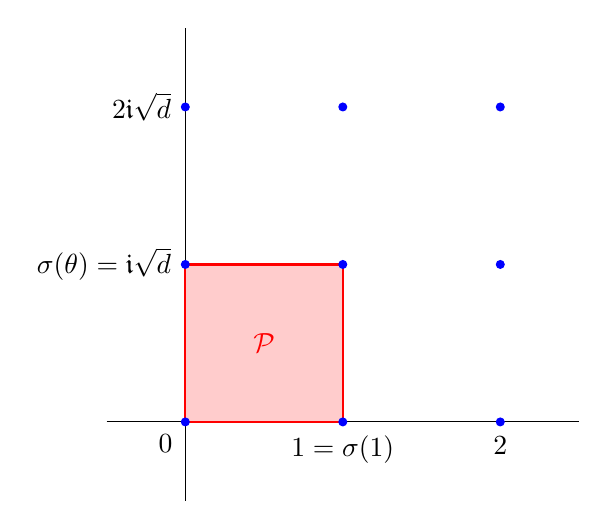
\begin{tikzpicture}[scale=2]
\draw (-0.5,0) -- (2.5,0);
\draw (0,-0.5) -- (0,2.5);
\draw[thick, fill, red, fill opacity=0.2] (0,0)--(1,0)--(1,1)--(0,1)--(0,0);
\node[circle, draw, fill, blue, inner sep=0.1em, label={below left:$0$}] at (0,0) {};
\node[circle, draw, fill, blue, inner sep=0.1em, label={below:$1=\sigma(1)$}] at (1,0) {};
\node[circle, draw, fill, blue, inner sep=0.1em, label={below:$2$}] at (2,0) {};
\node[circle, draw, fill, blue, inner sep=0.1em, label={left:$\sigma(\theta) = \im\sqrt{d}$}] at (0,1) {};
\node[circle, draw, fill, blue, inner sep=0.1em] at (1,1) {};
\node[circle, draw, fill, blue, inner sep=0.1em] at (2,1) {};
\node[circle, draw, fill, blue, inner sep=0.1em, label={left:$2\im\sqrt{d}$}] at (0,2) {};
\node[circle, draw, fill, blue, inner sep=0.1em] at (1,2) {};
\node[circle, draw, fill, blue, inner sep=0.1em] at (2,2) {};
\node[red] at (0.5,0.5) {$\mathcal{P}$};
\end{tikzpicture}
\caption{$d \nequiv 3 \mod 4$. $\covol \sigma(\o_K) = \sqrt{d}$}
\end{subfigure}
\begin{subfigure}{0.5\textwidth}
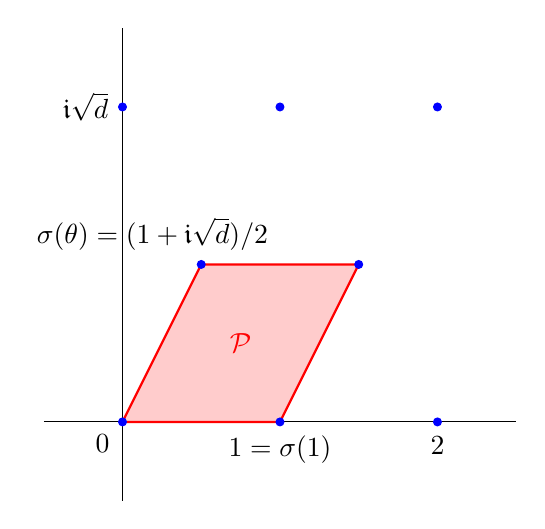
\begin{tikzpicture}[scale=2]
\draw (-0.5,0) -- (2.5,0);
\draw (0,-0.5) -- (0,2.5);
\draw[thick, fill, red, fill opacity=0.2] (0,0)--(1,0)--(1.5,1)--(0.5,1)--(0,0);
\node[circle, draw, fill, blue, inner sep=0.1em, label={below left:$0$}] at (0,0) {};
\node[circle, draw, fill, blue, inner sep=0.1em, label={below:$1=\sigma(1)$}] at (1,0) {};
\node[circle, draw, fill, blue, inner sep=0.1em, label={below:$2$}] at (2,0) {};
\node[circle, draw, fill, blue, inner sep=0.1em, label={[shift={(-.62,0)}]$\sigma(\theta) = (1+\im\sqrt{d})/2$}] at (0.5,1) {};
\node[circle, draw, fill, blue, inner sep=0.1em] at (1.5,1) {};
\node[circle, draw, fill, blue, inner sep=0.1em, label={left:$\im\sqrt{d}$}] at (0,2) {};
\node[circle, draw, fill, blue, inner sep=0.1em] at (1,2) {};
\node[circle, draw, fill, blue, inner sep=0.1em] at (2,2) {};
\node[red] at (0.75,0.5) {$\mathcal{P}$};
\end{tikzpicture}
\caption{$d \equiv 3 \mod 4$. $\covol \sigma(\o_K) = \frac12\sqrt{d}$}
\end{subfigure}
\end{figure}
The \emph{fundamental parallelepiped} attached the basis $\{e_i\}$ is $\mathcal{P} = \{\sum_{i=1}^n x_ie_i  : 0\leq x_i < 1\}$. The \emph{covolume} of $\Lambda$, $\covol(\Lambda)$, is the volume of $\mathcal{P}$, written $\vol(\mathcal{P}) = |\det(e_{ij})|$.

Note that in both cases above, $\covol(\sigma(\o_K)) = \frac12|d_K|^{\frac12}$.

Observe that if $x \in \R^n$ then there is a unique $y \in \P$ and $\lambda \in \Lambda$ such that $x = y +\lambda$, i.e. $\mathcal{P}$ is a set of coset representatives for $\Lambda \leq \R^n$

\begin{theorem}[Special Case of Minkowski's Theorem]
Let $X = \{z \in \C : |z|^2 \leq R\}$, and $\Lambda \subset \C$ be a lattice. If $\pi R \geq 4 \covol(\Lambda)$, then $X \cap \Lambda \neq \{0\}$.
\end{theorem}
\begin{theorem}
Let $I \subset \o_K \subset K = \Q(\sqrt{-d})$ be a non-zero ideal. Then there is some $\alpha \in I\setminus\{0\}$ with $\Nn_{K/\Q}(\alpha)\leq c_K \Nn(I)$, and $c_K = \frac{2}{\pi}|d_K|^{\frac12}$.
\end{theorem}
\begin{proof}
$I \subset \o_K \injection_\sigma \C$ is a lattice, and $\covol(\sigma(I)) = \Nn(I)\covol(\sigma(\o_K)) = \Nn(I)\frac{1}{2}|d_K|^{\frac12}$. Take $X$ as in \textbf{10.1}, and $R = \frac{2}{\pi}|d_K|^{\frac12}\Nn(I)$.

Then by \textbf{10.1}, $X \cap \sigma(I) \neq \{0\}$. But if $\alpha = u +v\sqrt{-d} \in K$, then $\sigma(\alpha) \in K \iff |\sigma(\alpha)|^2 = u^2+dv^2 \leq R \iff \Nn_{K/\Q}(\alpha) \leq R$. So there does exist some non-zero $\alpha$ in $I$ with $\Nn_{K/\Q}(\alpha) \leq R$.
\end{proof}

\begin{corollary}
Let $K = \Q(\sqrt{-d})$ be an imaginary quadratic. Then:
\begin{enumerate}
\item $Cl(K)$ is finite.
\item Every element of $Cl(K)$ contains an ideal of norm $\leq c_K = \frac{2}{\pi}|d_K|^{\frac12}$.
\item $Cl(K)$ is generated by the class of prime ideals of norm $\leq C_K$.
\end{enumerate}
\end{corollary}
\begin{proof}
\begin{itemize}
\item[2.] Let $I \subset \o_K$ be a non-zero ideal. Choose $J$ with $IJ = (\beta)$. Then by \textbf{10.2}, there is some $\alpha \in J \setminus \{0\}$ with $\Nn_{K/\Q}(\alpha) \leq c_K \Nn(J)$. Then $(\alpha) = JI'$ for some $I'$, and $\Nn(I') = \frac{\Nn((\alpha))}{\Nn(J)} = \frac{\Nn_{K/\Q}(\alpha)}{\Nn(J)} \leq c_K$, and $(\alpha\beta) = \alpha IJ = \beta JI'$, so $\alpha I = \beta I'$, i.e. $I' \simeq I$.
\end{itemize}
Then $(2.)\implies(3.)$ by writing $I' = \prod P_i$ as a product of primes of norm $\leq c_K$, and $(2.)\implies(1.)$ since the number of ideals of norm $\leq c_K$ is finite by \textbf{7.2}.
\end{proof}

\hspace*{-1em}\underline{Examples:}\\
$K = \Q(\im)$. Then $d_K = 4$, so every ideal class contains an ideal $I$ with norm $\leq c_K = \frac{2}{\pi}4^{1/2} = \frac{4}{\pi} < 2$, i.e. with norm 1, so $I = \o_K$. So $Cl(K)$ is trivial, and we have another proof that $\Z[i]$ is a PID.

$K = \Q(\sqrt{-5}$. We've seen already that $\o_K$ is not a PID. Let's compute $Cl(K)$. We have $d_K = -20$, so $c_K = \frac{2\sqrt{20}}{\pi} < \frac{9}{\pi} < 3$, so every ideal class contains an ideal of norm $\leq 2$. Recall that $(2) = (2, 1+\sqrt{-5})^2 = P^2, \Nn(P) = 2$. So the only ideals of norm $\leq 2$ are $\o_K$ and $P$, and hence $Cl(K)$ has order two, with elements $[\o_K], [P]$. 

$K = \Q(\sqrt{d})$. Then we have the two embeddings $\sigma_1,\sigma_2: \sqrt{d} \mapsto \pm \sqrt{d}$. So the lattice we get is generated by $\sigma(1) = (\sigma_1(1), \sigma_2(1)) = (1,1), \sigma(\sqrt{d}) = (\sqrt{d}, -\sqrt{d})$, which is indeed a basis for $\R^2$, and so $\sigma(\Z[\sqrt{d}])$ is indeed a lattice. Then $\Nn_{K/\Q}(\alpha) = \sigma_1(\alpha)\sigma_2(\alpha) \leq R$ if and only if $\sigma(\alpha)$ lies in the region bounded by $x_1x_2 = \pm R$.
\begin{figure}[H]
\centering
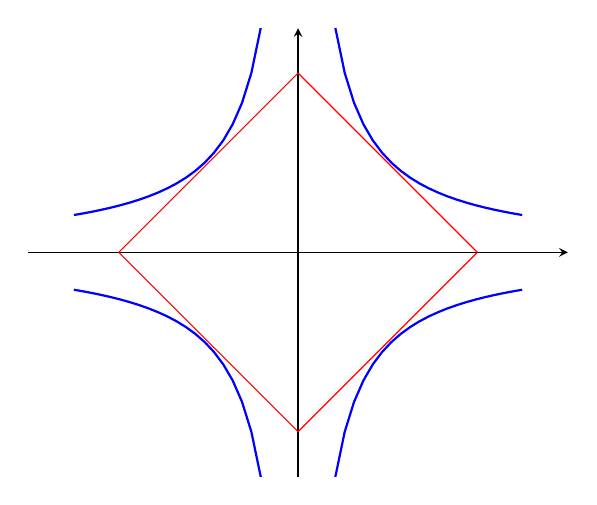
\begin{tikzpicture}
\begin{axis}[axis lines=middle, xmin=-3, xmax=3, ymin=-3, ymax=3, xtick=\empty, ytick=\empty, xticklabels=\empty, yticklabels=\empty, axis equal]
\addplot[blue, thick, domain=-3:0] (x, {1.5/x});
\addplot[blue, thick, domain=0:3] (x, {1.5/x});
\addplot[blue, thick, domain=-3:0] (x, {-1.5/x});
\addplot[blue, thick, domain=0:3] (x, {-1.5/x});
\addplot[red] coordinates{(-2.4,0)(0,2.4)};
\addplot[red] coordinates{(-2.4,0)(0,-2.4)};
\addplot[red] coordinates{(2.4,0)(0,2.4)};
\addplot[red] coordinates{(2.4,0)(0,-2.4)};
\draw[green!60!black] (axis cs: 0, 0) circle [radius=170];
\end{axis}
\end{tikzpicture}
\end{figure}
\begin{theorem}[Minkowski's Theorem]
Let $\Lambda \subset \R^n$ be a lattice, and $X \subset \R^n$ be a convex, measurable set that is symmetric about 0. Then if either:
\begin{itemize}
\item $\vol(X) > 2^n\covol(\Lambda)$
\item $\vol(X) \geq 2^n\covol(\Lambda)$ and $X$ is compact
\end{itemize}it must be the case that $X \cap \Lambda \neq\{0\}$.
\end{theorem}
Note the strict inequality in the first case versus the weak one in the second case. Before we can prove this we will need the following lemma:

\begin{lemma}[Blichfeldt's Lemma]
Let $\Lambda \subset \R^n$ be a lattice and $Y \subset \R^n$ be a measurable subset. If $\vol(Y)> \covol(\Lambda)$ there is $x, y \in Y$ with $x\neq y$ such that $x-y \in \Lambda$.
\end{lemma}
The idea behind this slightly messy proof is that we have a projection map $\pi:\R^n\to \R^n/\Lambda$, where $\vol(\R^n/\Lambda) = \covol(\Lambda) \geq \vol(\pi(Y))$,  but $\vol(Y) > \covol(\Lambda)$, and so $Y\to \pi(Y)$ is not 1-1.
\begin{proof}
For $\lambda \in \Lambda$, let $Y_{\lambda} = \{x \in Y : x-\lambda \in \mathcal{P}\} = Y \cap (\lambda+\mathcal{P})$. Then we have that $-\lambda + Y_{\lambda} = \{x-\lambda:x \in Y_\lambda\} \subset \mathcal{P}$.

Then $Y$ is the disjoint union of the $Y_{\lambda}$, since $\R^n = \coprod_{\lambda\in \Lambda} \lambda + \mathcal{P}$.

So $\vol(Y) = \sum \vol(Y_\lambda) = \sum \vol(-\lambda + Y_\lambda) > \vol(\mathcal{P})$, so the subsets $-\lambda + Y_\lambda$ cannot be disjoint, and so there is $x, y \in Y$ with $x - \lambda_1 = y-\lambda_2$. But then $x-y = \lambda_1-\lambda_2 \in \Lambda$.
\end{proof}

\begin{proof}[Proof of Minkowski]
Assume $\vol(X) > 2^n\covol(\Lambda) = \covol(2\lambda)$. Then by Blichfeldt, there is $x,y \in X$ with $0 \neq x - y \in 2\Lambda$. As $X$ is symmetric, $-y \in X$. As $X$ is convex, $\frac{x+(-y)}{2} \in X$, but also $\frac{x-y}{2} \in \Lambda\setminus \{0\}$.

Now suppose $X$ is compact and $\vol(X) = 2^n \covol(\Lambda)$. For $\delta > 0$, let $X_\delta = \{(1+\delta)x : x \in X\} \supset X$ as $X$ is convex and $0 \in X$. By the first part $X_{\delta} \cap \Lambda \neq \{0\}$ as $\vol(X_{\delta}) > 2^n\covol(\Lambda)$. 

$X_\delta$ is bounded, and $\Lambda = \bigoplus_{i=1}^n \Z e_i$ for a basis $(e_i)$ of $\R^n$, so $X_\delta \cap \Lambda$ is finite. $X$ is also closed, so $X = \bigcap_{\delta>0} X_\delta$, so $X \cap \Lambda= \bigcap_{\delta} (X_\delta \cap \Lambda) = X_{\delta'} \cap \Lambda$ for some $\delta' >0$, and so $X \cap \Lambda \neq \{0\}$.
\end{proof}

Now let $K$ be a number field, and order the embeddings $K \injection \C$ as $\sigma_1, \ldots, \sigma_r:K \injection \R; \sigma_{r+1},\ldots,\sigma_{r+2s}:K \injection \C$, with $\sigma_{r+s+i} = \overline{\sigma_{r+i}}\neq \sigma_{r+i}$.

Then the \emph{product} is an embedding $\sigma:K \injection \R^r\times \C^s \cong \R^n; \alpha\mapsto (\sigma_1(\alpha), \ldots, \sigma_{r+s}(\alpha))$.

\begin{proposition}
$\sigma(\o_K) \subset \R^n$ is a lattice of covolume $2^{-s}|d_K|^{\frac12}$.
\end{proposition}
\begin{proof}
Let $\omega_1, \ldots, \omega_n$ be an integral basis for $K$. Then $e_i = \sigma(\omega_i) \in \R^n$ is the vector $e_i = (\sigma_1(\omega_i), \ldots, \sigma_r(\omega_i), \mathfrak{Re}\,\sigma_{r+1}(\omega_i), \mathfrak{Im}\,\sigma_{r+1}(\omega_i), \ldots, \mathfrak{Im}\,\sigma_{r+1}(\omega_i)) = (e_{ij})_{1\leq j \leq n}$.

Then $\covol \sigma(\o_K) = |\det(e_{ij})|$. But:
\begin{align*}
\begin{pmatrix}
\sigma_j(\omega_i) \\ \bar{\sigma_j}(\omega_i)
\end{pmatrix} = \begin{pmatrix}
1 & \im \\ 1 & -\im
\end{pmatrix}\begin{pmatrix}
\mathfrak{Re}\,\sigma_j(\omega_i)\\\mathfrak{Im}\,\sigma_j(\omega_i)
\end{pmatrix}
\end{align*}
And so $\det(e_{ij}) = \pm\left(\frac{1}{-2\im}\right)^{-s}\det(\sigma_j(\omega_i))$, and so $\covol(\sigma(\o_K)) = 2^{-s}|\det(\sigma_j*\omega_i))| = 2^{-s}|d_K|^{\frac12}$.
\end{proof}

Then by \textbf{7.1} we can immediately deduce:
\begin{corollary}
Let $I \subset \o_K$ be a nonzero ideal. Then $\sigma(I)$ is a lattice of covolume $2^{-s}|\disc(I)|^{\frac12} = 2^{-s}\Nn(I)|d_K|^{\frac12}$.
\end{corollary}
This then lets us state the main theorem of this section:
\begin{theorem}[Minkowski Bound]
For any nonzero $I \subset \o_K$, there exists $0 \neq \alpha \in I$ with $|\Nn_{K/\Q}(\alpha)| \leq c_K\Nn(I)$, where:
\begin{align*}
c_k = \left(\frac{4}{\pi}\right)^s \frac{n!}{n^n}|d_K|^{\frac12}
\end{align*}
where $n = r+2s$ in the usual way.
\end{theorem}
Some special cases to be aware of: real quadratic fields give $c_K = \frac{1}{2}|d_K|^{\frac12}$, and imaginary quadratics give $\frac{2}{\pi}|d_K|^{\frac12}$.
\begin{proof}
We will first consider the case $K = \Q(\sqrt{d})$, $d > 0$. Then $\sigma:K \injection \R^2$ is given by $u+v\sqrt{d} \mapsto (u+v\sqrt{d}, u-v\sqrt{d})$. $\Nn_{K/\Q}(\alpha) = \sigma_1(\alpha)\sigma_2(\alpha) = u^2-dv^2$, and so $|\Nn_{K/\Q}(\alpha)| \leq R$ if and only if $\sigma(\alpha)$ lies in the region bounded by the hyperbolae $x_1x_2 = \pm R$.
\begin{center}
\begin{tikzpicture}
\begin{axis}[axis lines=middle, xmin=-3, xmax=3, ymin=-3, ymax=3, xtick=\empty, ytick=\empty, xticklabels=\empty, yticklabels=\empty]
\addplot[blue, thick, domain=-3:0] (x, {1.5/x});
\addplot[blue, thick, domain=0:3] (x, {1.5/x});
\addplot[blue, thick, domain=-3:0] (x, {-1.5/x});
\addplot[blue, thick, domain=0:3] (x, {-1.5/x});
\end{axis}
\end{tikzpicture}
\end{center}
To apply Minkowski's theorem, we need to choose a convex symmetric subset of this region, and for optimal bound we want it to have the largest possible area. This is the square with vertices $(\pm 2R^{\frac12},0),(0,\pm 2R^{\frac12})$, and area $8R$. Then Minkowski's theorem gives us a lattice point in this region if $8R \geq 4\covol \sigma(I) = 4|d_k|^{\frac12}\Nn(I)$.

Then taking $R = \frac12 |d_K|^{\frac12} \Nn(I)$, there is some $0 \neq \alpha \in I$ with $\Nn_{K/\Q}(\alpha)| \leq c_K \Nn(I)$, with $c_K = \frac{1}{2}|d_K|^{\frac12}$, the $c_K$ of the theorem if $(r,s) = (2,0)$

For the general case, we have $\sigma: K \injection \R^r \times \C^s \cong \R^{n}$. The quadratic cases suggest the following choice:
\begin{align*}
X = X_R = \{(x_1, \ldots, x_r, z_1, \ldots, z_s) \in \R^r\times \C^s | \sum |x_j| + 2 \sum |z_j| \leq nR^\frac{1}{n}\}
\end{align*}
Then the AM-GM inequality gives that:
\begin{align*}
\prod |x_j| \prod |z_j|^2 &\leq R\\
\sigma(\alpha) \in X_R \implies |\Nn_{K/\Q}(\alpha)|&\leq R
\end{align*}
It is an exercise to show that $X_R$ is convex and symmetric about $0$ and compact. It remains only to compute the volume of $X_R$ - see Lemma \textbf{10.10}.
\end{proof}
\begin{corollary}
Every ideal class of $K$ contains an ideal of norm $\leq c_K$. In particular, $Cl(K)$ is finite, generated by the classes of prime ideals of norm $\leq c_K$.
\end{corollary}
\begin{proof}
Word for word the same as \textbf{10.3}
\end{proof}
\begin{lemma}
\begin{align*}
\vol(X_r) = 2^r \left(\frac{\pi}{2}\right)^s \frac{n^n}{n!}R
\end{align*}
\end{lemma}
If we put this with Minkowski's theorem, we get Minkowski's bound.

\underline{Examples of using Minkowski's bound:}
\begin{itemize}
\item Let $K = \Q(\sqrt{-17})$, $d_K = -68$, $c_K = 2\frac{\sqrt{68}}{\pi}<2\frac{9}{3} = 6$, so $Cl(K)$ is generated by classes of prime ideals of norm $2,3$, or $5$, since if $P$ is prime of norm $p^2$ then $P$ would be $(p)$, so principal.

\begin{itemize}
\item $p=5$. $-17 \equiv -2$ which is not a square mod 5, so 5 is inert and there is no $P$ of norm $5$.
\item $p=3$. $-17 \equiv 1^2 \mod 3$, so $(3) = P_3P_3'$. Then we can compute $P_3 = (3, 1+\sqrt{-17}), P_3' = (3, 1-\sqrt{-17})$.
\item $p=2$. This is ramified as $-17 \nequiv 1 \mod 4$, so $(2) = P_2^2, P_2 = 2, 1+\sqrt{-17})$.
\end{itemize}
Note that none of $P_2, P_3, P_3'$ are principal as there is no solution of $u^2 + 17v^2 = 2$ or $3$ in the integers.

We have the relations $[P_2]^2 = 1 = [P_3][P_3']$ in the class group $Cl(K)$. To find more relations, we can do $P_3^2 = (3,1+\sqrt{-17})^2 = (9, 1+\sqrt{-17})$, which has norm 9. Now $\Nn_{K/\Q}(1+\sqrt{-17}) = 18$, and $1+\sqrt{-17} \in P_3^2$, and so $(1+\sqrt{-17}) = P_3^2 \times (\text{norm 2}) = P_2P_3^2$, as $P_2$ is the only ideal of norm 2. Hence in $Cl(K), [P_3]^2 = [P_2]^{-1} = [P_2]$. 

Hence $Cl(K)$ is cyclic of order 4 generated by $[P_3]$.

\item $K = \Q(\theta)$, for $\theta$ a root of $g = x^5 - x+1$, which is irreducible mod 5 and hence irreducible. We can show that $g$ has 1 real root, so $(r,s) = (1,2)$. The discriminant of $g$ is $2689 = 19\times 151$ is squarefree. So $\o_K = \Z[\theta]$. $c_K = 3.3\ldots$, and so $Cl(K)$ is generated by prime ideals of norm $\leq 3$. Dedekind's criterion says that there is a prime of norm $p$ if and only if $g$ has a root mod $p$. But $g$ has no root mod 2 or mod 3. So $Cl(K)$ is trivial.
\end{itemize}
It is known that $\#Cl(\Q(\sqrt{-d})) \to \infty$ as $d \to \infty$, and $Cl(K) \neq \{1\}$ for all $d > 163$). If $K = \Q(\sqrt{d})$, it is thought that there are infinitely many $d$ with $|Cl(K)| = 1$.

\example Compute $Cl(K)$ for $K = \Q(\sqrt{10})$.

The Minkowski constant $c_K = \frac12 \sqrt{40} = \sqrt{10} < 4$, so $Cl(K)$ is generated by classes of prime ideals of norm 2 or 3.
\begin{itemize}
\item $(2) = (2, \sqrt{10})^2 = P_2^2$
\item $(3) = (3, 1+\sqrt{10})(3, 1-\sqrt{10}) = P_3P_3'$
\end{itemize}
So $[P_2]^2 = [P_3][P_3'] = 1$ in $Cl(K)$. To get more relations, look at elements of $\o_K$ of small norm. Any relation between $[P_2]$ and $[P_3]$ is of the form $P_2^mP_3^n = (\alpha)$, where $\Nn_{K/\Q}(\alpha) = \pm 2^m 3^n$.
\begin{itemize}
\item $Nn_{K/\Q}(1+\sqrt{10}) = -9$, and $1+\sqrt{10} \in P_3 \implies P_3|(1+\sqrt{10})$. As $1+\sqrt{10} \notin P_3'$, we must have $P_3^2 = (1+\sqrt{10})$.
\item $\Nn_{K/\Q}(2+\sqrt{10}) = -6$, and $2+\sqrt{10} \in P_2 \cap P_3'$. So $(2+\sqrt{10}) = P_2P_3'$.
\end{itemize}
 Hence $[P_2] = [P_3] = [P_3']$ has order 1 or 2 in $Cl(K)$, so either $Cl(K) = \{1\}$ or $\Z/2\Z$. Is $P_2$ principal? If so $P = (u+v\sqrt{10})$, and $u^2-10v^2 = \pm 2$, so $u^2 \equiv \pm 2 \mod 5$, which is impossible. So $P_2$ is not principal and $Cl(K) \cong \Z/2\Z$.
 
We call the order of the class group $\#Cl(K)$ the \emph{class number} of $K$, and write $h_K$. If $K$ is an imaginary quadratic, then the ideal class group is closely related to the classes of binary quadratic forms of discriminant $d_K$.

\section{Units}
If $K$ is a number field, then we call the group of units $\o_K^{\ast}$, the multiplicative group of algebraic integers.
\begin{theorem}[Dirichlet's Unit Theorem]
$\o_K^{\ast}$ is finitely generated of rank $r+s-1$.
\end{theorem}
The torsion subgroup of $\o_K^{\ast}$ is the subgroup of elements of finite order in $K^{\ast}$, i.e. the roots of unity, as every root of unity is an algebraic integer. So this group is finite and therefore is \textit{cyclic} by Galois theory.

So this theorem says that there are $\epsilon_1, \ldots, \epsilon_{r+s-1} \in \o_K^{\ast}$ such that every $\epsilon \in \o_K^{\ast}$ can be uniquely written as $\epsilon = \zeta \epsilon_1^{a_1} \ldots \epsilon_{r+s-1}^{a_{r+s-1}}$ for $a_i \in \Z$, where $\zeta$ is a root of unity in $K$.

\example $K = \Q(\sqrt{d})$ quadratic, $\o_K = \{u+v\sqrt{d}\}$. Recall if $\alpha \in \o_K$ then $\alpha \in \o_K^{\ast} \iff \Nn_{K/\Q}(\alpha) = \pm 1 = u^2-dv^2$ in this case. 

\begin{itemize}
\item $K = \Q(\sqrt{d})$ imaginary quadratic. $\alpha \in \o_K^\ast \iff u^2-dv^2 = 1$, so $\o_K^{\ast}$ is finite, and $r+s-1 = 0+1-1 = 0$. It is easy to check that $\o_K^{\ast} = \{\pm 1\}$ except in the case $K = \Q(\sqrt{-1})$ or $\Q(\sqrt{-3})$, where $\ord(\o_K^\ast) = 4$ or $6$ respectively.

\item $K = \Q(\sqrt{d})$ real quadratic. Then we get \emph{Pell's Equation} $u^2-dv^2 = 1$, and by Part II Number Theory, there are infinitely many solutions for fixed $d > 1$, and so $\o_K^{\ast}$ is infinite. In fact we can be more precise:
\end{itemize}
\begin{theorem}
Let $K = \Q(\sqrt{d}) \subset \R$ for $d>0$ squarefree. Then there exists a unique smallest $\epsilon \in \o_K^\ast$ with $\epsilon > 1$, called the \emph{fundamental unit}, and $\o_K^\ast = \{\pm \epsilon^m : m \in \Z\}$.
\end{theorem}
\begin{proof}
Take as known that $\o_K^\ast$ is infinite - another proof of this will follow. Then the only roots of unity in $K$ are $\pm 1$ since $K \subset \R$. Let $\epsilon \in \o_K^{\ast} \setminus \{\pm 1\}$, $\epsilon = u +v\sqrt{d}$. We then claim claim that $\epsilon > 1$ if and only if both $u, v > 0$. 

Indeed, as $\epsilon$ is unit, i.e. $u^2-dv^2 = \pm 1$, all of $\{\pm u \pm v \sqrt{d}\} = \{\pm \epsilon, \pm 1/\epsilon\}$ are units, and exactly one of them lies in the each of the intervals $(-\infty, -1),(-1,0),(0,1),(1, \infty)$. So $\epsilon > 1 \iff \epsilon$ is the largest of these four, and so $\epsilon \in (1, \infty)$.

So now choose $\epsilon \in \o_K^\ast$, $\epsilon > 1$ with $v$ minimal. It is then easy to see that $\epsilon$ is minimal, and then if $\epsilon' \in \o_K^\ast$, $\epsilon' > 1$ and so there exists $m \geq 1$ with $\epsilon^m \leq \epsilon' < \epsilon^{m+1}$. Then $1 \leq \epsilon'/\epsilon^m < \epsilon$, so by minimality, $\epsilon'/\epsilon^m = 1$, So the set of units $>1$ is precisely $\{\epsilon^m : m \geq 1\}$. Repeating this for each of the four intervals, we see that $\o_K^{\ast} = \{\pm \epsilon^m : m \in \Z\}$.
\end{proof}
\begin{proof}[Direct proof without using continued fractions]
We first construct lots of elements of $K$ of bounded norm, using the following lemma:
\begin{lemma}
If $R \geq |d_K|^{\frac12}$, there are infinitely many $\alpha \in \o_K$ with $|\Nn_{K/\Q}(\alpha)| \leq R$.
\end{lemma}
Assuming this, using the fact that there are only finitely many ideals of norm $\leq R$, we have that $\exists \alpha \neq \beta \in \o_K$ with $(\alpha) = (\beta)$, and then $\alpha/\beta \in \o_K^{\ast}$.
\begin{proof}[Proof of Lemma]
$\sigma : K \injection \R^2; \sqrt{d} \mapsto (\sqrt{d}, -\sqrt{d})$. Consider the rectangle $Y_\delta = [-R/\delta, R/\delta] \times [-\delta, \delta]$. 
\begin{center}
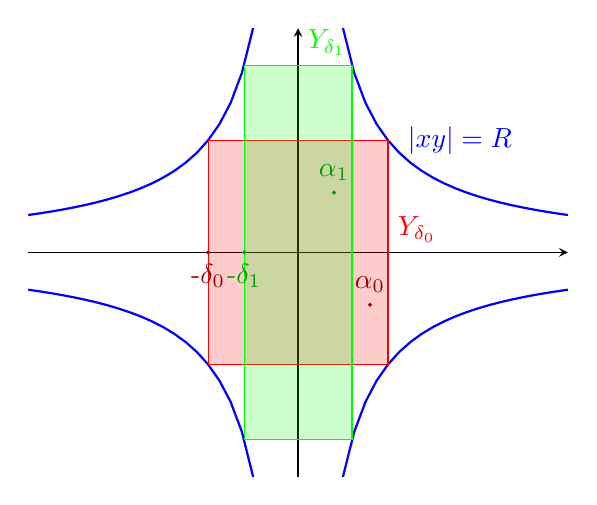
\begin{tikzpicture}
\begin{axis}[axis lines=middle, xmin=-3, xmax=3, ymin=-3, ymax=3, xtick=\empty, ytick=\empty, xticklabels=\empty, yticklabels=\empty]
\addplot[blue, thick, domain=-3:0] (x, {1.5/x});
\addplot[blue, thick, domain=0:3] (x, {1.5/x});
\addplot[blue, thick, domain=-3:0] (x, {-1.5/x});
\addplot[blue, thick, domain=0:3] (x, {-1.5/x});
\draw[red, fill, fill opacity=0.2] (axis cs:-1,-1.5)--(axis cs:-1,1.5)--(axis cs:1,1.5)--node[above right, red, opacity=1] {$Y_{\delta_0}$}(axis cs:1,-1.5)--(axis cs:-1,-1.5);
\node[red!60!black, circle, draw, fill, inner sep=0.01em, minimum size=0.1em, label={[red!60!black]above:$\alpha_0$}] at (axis cs: 0.8, -0.7) {};
\draw[green, fill, fill opacity=0.2] (axis cs:-.6,-2.5)--(axis cs:-.6,2.5)--node[above right, opacity=1] {$Y_{\delta_1}$}(axis cs:.6,2.5)--(axis cs:.6,-2.5)--(axis cs:-.6,-2.5);
\node[green!60!black, circle, draw, fill, inner sep=0.01em, minimum size=0.1em, label={[green!60!black]above:$\alpha_1$}] at (axis cs:0.4, 0.8) {};
\node[red!60!black, circle, draw, fill, inner sep=0.01em, minimum size=0.1em, label={[red!60!black]below:-$\delta_0$}] at (axis cs:-1, 0) {};
\node[green!60!black, circle, draw, fill, inner sep=0.01em, minimum size=0.1em, label={[green!60!black]below:-$\delta_1$}] at (axis cs:-.6, 0) {};
\node[blue] at (axis cs:1.8,1.5) {$|xy|=R$};
\end{axis}
\end{tikzpicture}
\end{center}
$4R = \vol(Y_\delta) \geq 4 \covol \sigma(\o_K) = 4|d_K|^{\frac12}$. Then take $\delta = \delta_0 = 1$. By Minkowski, there exists $\alpha_0 \in \o_K \setminus \{0\}$ with $\sigma(\alpha) \in Y_\delta$.

Hence $|\Nn_{K/\Q}(\alpha_0)| \leq R$, and $|\sigma_1(\alpha_0)| \leq \delta_0$. Now let $0 < \delta_1 < |\sigma_1(\alpha_0)| \implies \alpha_1 \in \o_K \setminus \{0\}$, with $|\Nn_{K/\Q}(\alpha_1)|\leq R$ and $|\sigma_1(\alpha_1)| \leq \delta_1 < |\sigma_1(\alpha_0)|$. Continuing, we get an infinite sequence of $\alpha_0, \alpha_1, \ldots$ of distinct elements of $\o_K$ with $|\Nn_{K/\Q}(\alpha_j)|\leq R$.
\end{proof}
\end{proof}
\begin{lemma}
A subgroup $\Lambda \subset \R^n$ is a lattice if and only if:
\begin{enumerate}
\item It spans $\R^n$
\item For every bounded $X \subset \R^n$, $X\cap \Lambda$ is finite.
\end{enumerate}
\end{lemma}
A subgroup satisfying the second condition is called a \emph{discrete subgroup}, because the induced topology on $\Lambda$ is discrete. In this case, if $V \subset \R^n$ is the span of $\Lambda$, the lemma implies that $\Lambda$ is a lattice in $V \cong \R^m$ for some $m \leq n$, so is freely generated by $m \leq n$ linearly independent elements.
\begin{proof}
Suppose $\Lambda \subset \R^n$ is a lattice, so is $=\bigoplus_{i=1}^n \Z e_i$, with $(e_i)$ a basis. Then there is invertible $u : \R^n \to \R^n$ such that $u(\Lambda) = \Z^n$. Then $X$ bounded if and only if $u(X)$ is bounded, and if so, $u(X) \cap \Z^n$ is clearly finite.

Conversely, assume the two conditions. Then $\Lambda$ contains a basis for $\R^n$ by \textit{1.}, so after a change of basis we may assume $\Lambda \supset \Z^n$. Then let $S = \{x = (x_i)\in \Lambda | 0 \leq x_i < 1 \forall i\}$. Then $\Lambda = \{x+\lambda : x \in S, \lambda \in \Z^n\}$, i.e. $S$ is a set of coset representatives of $\Z^n \leq \Lambda$. Now $S$ is finite, so $(\Lambda : \Z^n) = d < \infty$, and so $\frac1d\Z^n \supset \Lambda$. Then by GRM, $\Lambda$ is free abelian of rank $n$, so is $\sum \Z e_i$, but since $\Lambda$ spans $\R^n$, the $e_i$ are independent, so $\Lambda = \bigoplus \Z e_i$, a lattice.
\end{proof}
\begin{lemma}
Let $C > 0$, $K$ an algebraic field. Then $\{\alpha \in \o_K : \forall i |\sigma_i(\alpha)| \leq C\}$ is finite.
\end{lemma}
\begin{proof}
Consider the characteristic polynomial of $\alpha$:
\begin{align*}
\prod_i(x-\sigma_i(\alpha)) &= x^n + \sum_{r=1}^n c_r x^{n-r} \\
&= x^n + \sum_{r=1}^n (-1)^r \sum_{i_1<\ldots<i_r} \sigma_{i_1}(\alpha)\ldots\sigma_{i_r}(\alpha) x^{n-r}
\end{align*}
As $c_r \in \Z$, $|c_r| \leq \binom{n}{r}C^r$, there are only finitely many such characteristic polynomials.
\end{proof}
\begin{corollary}
The group of roots of unity in $K$ is finite, so cyclic by Galois theory.
\end{corollary}
\begin{proof}
Roots of unity are algebraic integers as they satisfy $x^n-1$, and satisfy $|\sigma_i(\alpha)| = 1$.
\end{proof}
To show $\o_K^{\ast}$ is finitely generated, we use lattice methods by mapping into some $\R^m$, so we will take logarithms.

We define the \emph{logarithmic embedding} $\mathscr{L}:K^{\ast} \to \R^{r+s}$, given by:
\begin{align*}
\mathscr{L}(\alpha) = (\mathscr{L}(\alpha)_i)_{1\leq i\leq r+s} \in \R^{r+s}\\
\mathscr{L}(\alpha)_i = \begin{cases} \log|sigma_i(\alpha) & 1 \leq i \leq r \\ 2\log|\sigma_i(\alpha)| & r+1 \leq i \leq r+s\end{cases}
\end{align*}
Then we have the following properties of $\mathscr{L}$:
\begin{enumerate}
\item $\mathscr{L}$ is a homomorphism.
\item $\alpha in K^{\ast} \implies \sum_{i=1}^{r+s} \mathscr{L}(\alpha)_i = \log |\Nn_{K/\Q}(\alpha)|$, since:
\begin{align*}
\log |\Nn_{K/\Q}(\alpha)| &= \sum_{i=1}^n \log |\sigma_i(\alpha)|\\
&= \sum_{i=1}^r \log |\sigma_i(\alpha)| + \sum_{i=1}^s \log |\sigma_{r+i}(\alpha)| + \log |sigma_{r+s+i}(\alpha)|\\
&= \sum_{i=1}^{r+s} \mathscr{L}(\alpha)_i
\end{align*}
\item $\alpha \in \o_K^\ast \implies \mathscr{L}(\alpha) \in \R^{r+s,0}\coloneqq \{(x_i) \in \R^{r+s} : \sum x_i = 0\}$, and $\mathscr{L}(\alpha) = 0$ if $\alpha$ is a root of unity.
\end{enumerate}
\begin{proposition}
\item
\begin{enumerate}
\item $\ker \mathscr{L} \cap \o_K^\ast$ is the subgroup of roots of unity in $K$.
\item $\mathscr{L}(\o_K^\ast)$ is a discrete subgroup of $\R^{r+s,0}$.
\end{enumerate}
\end{proposition}
\begin{proof}
Let $M >0$ and consider $Z = \{(x_i) \in \R^{r+s} : \forall i |x_i|\leq M\}$. Then $\mathscr{L}(\alpha) \in Z \iff e^{-M} \leq |\sigma_i(\alpha)|\leq e^M$ for $i \leq r$, and the same with $|\sigma_i(\alpha)|^2$ for $i >r$.

So by lemma \textbf{11.5} $S = \{\alpha \in \o_K^\ast : \mathscr{L}(\alpha) \in Z\}$ is finite. As $0 \in Z, S \supset \ker \mathscr{L} \cap \o_K^\ast$, so $\ker \mathscr{L} \cap \o_K^\ast$ is finite. By the third property above, we have \textit{1.} $S$ is finite, so $\mathscr{L}(\o_K^\ast)\cap Z$ is finite for all $M$, yielding \textit{2.}
\end{proof}
\begin{corollary}
$\o_K^\ast$ is finitely generated of rank $\leq r+s-1$.
\end{corollary}
\begin{proof}
$\mathscr{L}(\o_K^\ast)$ is a discrete subgroup of $\R^{r+s}$, contained in $\R^{r+s,0}$. So it is generated by $e_1, \ldots, e_t \in \R^{r+s, 0}$ linearly independent, for some $0 \leq t \leq r+s-1$. Choose $\epsilon_1, \ldots, \epsilon_t \in \o_K^\ast$ with $\mathscr{L}(\epsilon_i) = e_i$. Then for any $\epsilon \in \o_K^\ast$, $\mathscr{L}(\epsilon) = \sum_{i=1}^t m_ie_i$ for some unique $(m_i) \in \Z^t$, and hence $\epsilon/(\epsilon_1^{m_1}\ldots\epsilon_t^{m_t} = \zeta$ satisfies $\mathscr{L}(\zeta) = 0$, i.e. $\zeta$ is a root of unity. So $\o_K^\ast = \{\zeta \epsilon_1^{m_1}\ldots \epsilon_t^{m_t} : \zeta$ a root of unity, $m_i \in \Z\}$.
\end{proof}
Dirichlet's unit theorem says that, moreover, $\rank \o_K^\ast = r+s-1$. Note that $r+s-1 = 0$ in precisely 2 cases:
\begin{itemize}
\item $(r,s) = (1,0)$ in which case $K = \Q$
\item $(r,s) = (0,1)$ in which case $K = \Q(\sqrt{-d})$
\end{itemize}
So to prove the unit theorem, we will have to show:
\begin{theorem}
$\mathscr{L}(\o_K^\ast)$ is a lattice in $\R^{r+s, 0}$.
\end{theorem}
\end{document}
